%Version 3.1 December 2024
% See section 11 of the User Manual for version history
%
%%%%%%%%%%%%%%%%%%%%%%%%%%%%%%%%%%%%%%%%%%%%%%%%%%%%%%%%%%%%%%%%%%%%%%
%%                                                                 %%
%% Please do not use \input{...} to include other tex files.       %%
%% Submit your LaTeX manuscript as one .tex document.              %%
%%                                                                 %%
%% All additional figures and files should be attached             %%
%% separately and not embedded in the \TeX\ document itself.       %%
%%                                                                 %%
%%%%%%%%%%%%%%%%%%%%%%%%%%%%%%%%%%%%%%%%%%%%%%%%%%%%%%%%%%%%%%%%%%%%%

%%\documentclass[referee,sn-basic]{sn-jnl}% referee option is meant for double line spacing

%%=======================================================%%
%% to print line numbers in the margin use lineno option %%
%%=======================================================%%

%%\documentclass[lineno,pdflatex,sn-basic]{sn-jnl}% Basic Springer Nature Reference Style/Chemistry Reference Style

%%=========================================================================================%%
%% the documentclass is set to pdflatex as default. You can delete it if not appropriate.  %%
%%=========================================================================================%%

%%\documentclass[sn-basic]{sn-jnl}% Basic Springer Nature Reference Style/Chemistry Reference Style

%%Note: the following reference styles support Namedate and Numbered referencing. By default the style follows the most common style. To switch between the options you can add or remove "Numbered" in the optional parenthesis.
%%The option is available for: sn-basic.bst, sn-chicago.bst%  
 
%%\documentclass[pdflatex,sn-nature]{sn-jnl}% Style for submissions to Nature Portfolio journals
%%\documentclass[pdflatex,sn-basic]{sn-jnl}% Basic Springer Nature Reference Style/Chemistry Reference Style
\documentclass[pdflatex,sn-mathphys-num]{sn-jnl}% Math and Physical Sciences Numbered Reference Style
%%\documentclass[pdflatex,sn-mathphys-ay]{sn-jnl}% Math and Physical Sciences Author Year Reference Style
%%\documentclass[pdflatex,sn-aps]{sn-jnl}% American Physical Society (APS) Reference Style
%%\documentclass[pdflatex,sn-vancouver-num]{sn-jnl}% Vancouver Numbered Reference Style
%%\documentclass[pdflatex,sn-vancouver-ay]{sn-jnl}% Vancouver Author Year Reference Style
%%\documentclass[pdflatex,sn-apa]{sn-jnl}% APA Reference Style
%%\documentclass[pdflatex,sn-chicago]{sn-jnl}% Chicago-based Humanities Reference Style

%%%% Standard Packages
%%<additional latex packages if required can be included here>

\usepackage[utf8]{inputenc}%
\usepackage{graphicx}%
\usepackage{multirow}%
\usepackage{amsmath,amssymb,amsfonts}%
\usepackage{amsthm}%
\usepackage{mathrsfs}%
\usepackage[title]{appendix}%
\usepackage{xcolor}%
\usepackage{textcomp}%
\usepackage{manyfoot}%
\usepackage{booktabs}%
\usepackage{tcolorbox}%
\usepackage{pdflscape}%
\usepackage{tabularx}%
\usepackage{makecell}%
\usepackage{array}
\usepackage{tabularx}  
\newcommand{\cmark}{\ensuremath{\checkmark}}
\newcommand{\xmark}{\ensuremath{\times}}
\newcommand{\partialcmark}{\textcolor{yellow}{\ensuremath{\checkmark^{*}}}}

\newcolumntype{L}[1]{>{\raggedright\arraybackslash}p{#1}}
\newcolumntype{Y}{>{\centering\arraybackslash}X}
%%%%

%%%%%=============================================================================%%%%
%%%%  Remarks: This template is provided to aid authors with the preparation
%%%%  of original research articles intended for submission to journals published 
%%%%  by Springer Nature. The guidance has been prepared in partnership with 
%%%%  production teams to conform to Springer Nature technical requirements. 
%%%%  Editorial and presentation requirements differ among journal portfolios and 
%%%%  research disciplines. You may find sections in this template are irrelevant 
%%%%  to your work and are empowered to omit any such section if allowed by the 
%%%%  journal you intend to submit to. The submission guidelines and policies 
%%%%  of the journal take precedence. A detailed User Manual is available in the 
%%%%  template package for technical guidance.
%%%%%=============================================================================%%%%

%% as per the requirement new theorem styles can be included as shown below
\theoremstyle{thmstyleone}%
\newtheorem{theorem}{Theorem}%  meant for continuous numbers
%%\newtheorem{theorem}{Theorem}[section]% meant for sectionwise numbers
%% optional argument [theorem] produces theorem numbering sequence instead of independent numbers for Proposition
\newtheorem{proposition}[theorem]{Proposition}% 
%%\newtheorem{proposition}{Proposition}% to get separate numbers for theorem and proposition etc.

\theoremstyle{thmstyletwo}%
\newtheorem{example}{Example}%
\newtheorem{remark}{Remark}%

\theoremstyle{thmstylethree}%
\newtheorem{definition}{Definition}%

\raggedbottom
%%\unnumbered% uncomment this for unnumbered level heads

\begin{document}

\title[Article Title]{
    %A Survey of Multimodal XAI in Healthcare: \newline From architectures classification to an action-centered framework OR \\
    %A Survey of Multimodal XAI for Healthcare Decision-Making OR \\
    %A Survey and Benchmark of Multimodal XAI for Clinical Applications
    
%    A Survey of Multimodal XAI for Healthcare Decision-Making
%A Survey of Multimodal XAI in Healthcare:\\ From Architectures Classification to an Action-Centered Framework}
%A Review of Multimodal Explainable AI in Healthcare: An Action-Centered Framework for Clinical Decision Support
A Review of Multimodal XAI in Healthcare: Toward Action-Centered Explainability for Clinical Decision Support}
%%=============================================================%%
%% GivenName	-> \fnm{Joergen W.}
%% Particle	-> \spfx{van der} -> surname prefix
%% FamilyName	-> \sur{Ploeg}
%% Suffix	-> \sfx{IV}
%% \author*[1,2]{\fnm{Joergen W.} \spfx{van der} \sur{Ploeg} 
%%  \sfx{IV}}\email{iauthor@gmail.com}
%%=============================================================%%

\author*[1,2]{\fnm{First} \sur{Author}}\email{iauthor@gmail.com}

\author[2,3]{\fnm{Second} \sur{Author}}\email{iiauthor@gmail.com}
\equalcont{These authors contributed equally to this work.}

\author[1,2]{\fnm{Third} \sur{Author}}\email{iiiauthor@gmail.com}
\equalcont{These authors contributed equally to this work.}

\affil*[1]{\orgdiv{Department}, \orgname{Organization}, \orgaddress{\street{Street}, \city{City}, \postcode{100190}, \state{State}, \country{Country}}}

\affil[2]{\orgdiv{Department}, \orgname{Organization}, \orgaddress{\street{Street}, \city{City}, \postcode{10587}, \state{State}, \country{Country}}}

\affil[3]{\orgdiv{Department}, \orgname{Organization}, \orgaddress{\street{Street}, \city{City}, \postcode{610101}, \state{State}, \country{Country}}}

%%==================================%%
%% Sample for unstructured abstract %%
%%==================================%%

\abstract{
%Clinical adoption of AI in healthcare is hindered by a critical transparency gap: multimodal models integrating medical images, clinical notes, and genomic data remain opaque to clinicians, limiting their ability to trust and act upon model outputs. Multimodal eXplainable Artificial Intelligence (MXAI) methods have rapidly advanced in healthcare research, yet they remain weakly aligned with the requirements of healthcare decision-making. Existing surveys primarily categorize explanations by their generation mechanisms (ante-hoc vs. post-hoc), overlooking how explanations are actually used to support clinical decisions. \\
Clinical adoption of AI in healthcare is hindered by a transparency gap: multimodal models remain opaque to clinicians, and existing MXAI surveys categorize methods by generation mechanism (ante-hoc vs. post-hoc) rather than by how explanations support clinical decisions. 
%In this survey, we examine MXAI through the lens of healthcare decision-making and introduce the Action-Centered Explainability (ACE) framework, which maps five clinical actions—triage, diagnosis, treatment selection, audit, and monitoring, to their corresponding explanation requirements, each associated with distinct safety-critical properties. We survey over fifty methods, twelve datasets, and four evaluation frameworks, reviewing existing MXAI approaches through this action-centered lens and identifying critical gaps between current practice and clinician needs.
We introduce the Action-Centered Explainability (ACE) framework, mapping five clinical actions—triage, diagnosis, treatment selection, audit, and monitoring—to their explanation requirements. To support this framework, we complement the survey with a controlled benchmark illustrating how different MXAI methods satisfy these action-specific requirements under distribution shift.

%We introduce the Action-Centered Explainability (ACE) framework, mapping five clinical actions—triage, diagnosis, treatment selection, audit, and monitoring—to their explanation requirements, and survey over fifty methods, twelve datasets, and four evaluation frameworks through this lens.
%In this survey, we examine MXAI through the lens of healthcare decision-making and introduce the Action-Centered Explainability (ACE) framework, which maps clinical decisions—such as triage, diagnosis, treatment selection, audit, and monitoring—to their corresponding explanation requirements.
%We complement this survey with a controlled multimodal benchmark to operationalize key evaluation dimensions relevant to decision support. Using a reproducible DermaMNIST-based setting with synthetic clinical covariates and a controlled spurious hospital shift, our experiments show that intrinsic attention achieves the lowest latency, while perturbation-based methods remain significantly slower and saliency approaches exhibit measurable cross-modal leakage. 
%\textcolor{red}{In an expanded controlled benchmark with 500 OOD cases, 20 random seeds, and a grid of causal-invariance weights, causal training improved mean OOD accuracy from 0.604 to 0.753 and reduced the generalization gap from 0.252 to 0.091, with bootstrap confidence intervals and paired statistical tests supporting the robustness of the effect.
A controlled benchmark (500 OOD cases, 20 seeds) shows that causal training improves OOD accuracy from 0.604 to 0.753 (gap: $0.252 \to 0.091$), intrinsic attention achieves the lowest latency, and saliency methods exhibit cross-modal leakage. 
These results reinforce the central ACE claim: MXAI methods should not be selected by explainer family alone, but by whether they satisfy the latency, causal validity, stability, fairness, and traceability requirements of the clinical action they support.
%Based on these insights, we reorganize MXAI methods, datasets, and evaluation protocols around decision-oriented requirements, namely latency, causal validity, stability, counterfactual usefulness, and auditability. Rather than cataloging explainers by algorithmic family, this work provides clinicians and system designers with a structured, empirically grounded roadmap for selecting and evaluating MXAI methods according to the clinical action they must support.
Rather than cataloging explainers by algorithmic family, this work provides clinicians and system designers with an empirically grounded roadmap for selecting MXAI methods according to the clinical action they must support. 

\textcolor{red}{ Across both the controlled OOD benchmark and the six-domain ACE stress-test suite, no explainer dominated all clinical actions: low-latency methods were strongest for triage-like workflows, while intervention-based or perturbational methods were more informative for diagnosis, treatment reasoning, and audit.}

%Moreover, enforcing causal invariance improves out-of-distribution robustness and reduces reliance on spurious features, highlighting the importance of intervention-aware explanations for reliable decision-making. 
%Based on these insights, we reorganize MXAI methods, datasets, and evaluation protocols around decision-oriented requirements, namely latency, causal validity, stability, counterfactual usefulness, and auditability. Rather than merely cataloging explainers, this work provides a clinically grounded roadmap for MXAI systems that are interpretable, empirically stress-tested, and closer to real-world deployment constraints.


%%================================%%
%% Sample for structured abstract %%
%%================================%%

% \abstract{\textbf{Purpose:} The abstract serves both as a general introduction to the topic and as a brief, non-technical summary of the main results and their implications. The abstract must not include subheadings (unless expressly permitted in the journal's Instructions to Authors), equations or citations. As a guide the abstract should not exceed 200 words. Most journals do not set a hard limit however authors are advised to check the author instructions for the journal they are submitting to.
% 
% \textbf{Methods:} The abstract serves both as a general introduction to the topic and as a brief, non-technical summary of the main results and their implications. The abstract must not include subheadings (unless expressly permitted in the journal's Instructions to Authors), equations or citations. As a guide the abstract should not exceed 200 words. Most journals do not set a hard limit however authors are advised to check the author instructions for the journal they are submitting to.
% 
% \textbf{Results:} The abstract serves both as a general introduction to the topic and as a brief, non-technical summary of the main results and their implications. The abstract must not include subheadings (unless expressly permitted in the journal's Instructions to Authors), equations or citations. As a guide the abstract should not exceed 200 words. Most journals do not set a hard limit however authors are advised to check the author instructions for the journal they are submitting to.
% 
% \textbf{Conclusion:} The abstract serves both as a general introduction to the topic and as a brief, non-technical summary of the main results and their implications. The abstract must not include subheadings (unless expressly permitted in the journal's Instructions to Authors), equations or citations. As a guide the abstract should not exceed 200 words. Most journals do not set a hard limit however authors are advised to check the author instructions for the journal they are submitting to.
}

\keywords{
%Explainable, Interpretable, Multimodal, Artificial Intelligence, medical}
Multimodal Explainable AI, Clinical Decision Support, Action-Centered Explainability, Causal Inference }
%%\pacs[JEL Classification]{D8, H51}

%%\pacs[MSC Classification]{35A01, 65L10, 65L12, 65L20, 65L70}

\maketitle

\section{Introduction}\label{sec1}

The rapid integration of Artificial Intelligence into healthcare promises transformative advances in early disease detection and personalized treatment, yet the "black box" nature of multimodal models (combining medical images, clinical notes, and genomic data) poses a critical barrier to clinical adoption \cite{article}. In particular, the lack of transparency limits clinicians' ability to trust, validate, and act upon model outputs in real decision-making contexts.
Existing surveys such as \cite{rodis2024multimodalexplainableartificialintelligence} and \cite{SADEGHI2024109370} primarily categorize MXAI methods by generation mechanisms (ante-hoc vs. post-hoc), overlooking how explanations are actually used to support clinical decisions. Consequently, this technical focus creates a 'utility gap,' where algorithmic transparency does not translate into actionable insights for diverse medical tasks ranging from rapid triage in emergency departments to the forensic requirements of clinical audits.
Multimodal Explainable AI (MXAI) addresses this challenge by illuminating the decision-making process of these complex systems, making them interpretable and justifiable to clinicians. 
However, existing MXAI approaches often emphasize technical interpretability without explicitly considering how explanations support clinical decisions.
For instance, an MXAI system diagnosing lung conditions could identify computed tomography (CT) anomalies and correlate them with documented smoking history and relevant biomarkers, providing holistic explanations that build trust and facilitate acceptance \cite{Gaube2023,Niu2025}. 
Yet, such explanations remain difficult to operationalize unless they are aligned with specific clinical actions.
This survey provides a comprehensive overview of MXAI in healthcare, covering foundational XAI concepts, multimodal architectures, state-of-the-art methods, benchmark datasets, evaluation metrics, and critical challenges including scalability, causality, fairness, and human-centricity. Since 2024, the rapid deployment of multimodal foundation models (e.g., Med-PaLM, MedCLIP, GPT-4V) has intensified the need for robust explainability mechanisms to ensure clinical safety and regulatory compliance with emerging FDA and EU AI Act requirements \cite{wang2022medclipcontrastivelearningunpaired,liu2023holisticevaluationgpt4vbiomedical,fda2025draft,VANKOLFSCHOOTEN2024105152}. 
%These systems are increasingly integrated into clinical workflows, where explanations must meet strict requirements in terms of reliability, latency, and accountability. We examine practical deployment issues and limitations of current approaches, concluding with a roadmap for future research to advance transparent, trustworthy, and effective AI systems in healthcare.
We examine practical deployment issues and limitations of current approaches, concluding with a roadmap for future research. 

%In particular, we emphasize the gap between existing explainability methods and the needs of real-world decision support. \textbf{Unlike prior surveys, this work argues that the ante-hoc/post-hoc taxonomy is structurally misaligned with clinical decision support.} 
%While widely adopted in the literature, this distinction reflects algorithmic properties rather than end-user requirements. Clinicians do not choose explanations based on whether they are embedded in a model or applied afterward \cite{pmlr-v106-tonekaboni19a}; they ask: ``Is this case urgent?'', ``Why this diagnosis?'', ``Why this treatment?'', ``Can I defend this decision in court?'', ``Is the model still reliable after 6 months?'' 
%These questions correspond to distinct decision-making contexts that require different types of explanations. Each question demands distinct explanation properties---speed, causality, counterfactuals, stability, temporal consistency---that current MXAI taxonomies do not foreground \cite{pmlr-v106-tonekaboni19a,gniadek2023framework} . As a result, existing frameworks fail to capture the practical requirements of clinical use.
Unlike prior surveys, this work argues that the ante-hoc/post-hoc taxonomy is structurally misaligned with clinical decision support: it reflects algorithmic properties rather than end-user requirements [10, 11]. Clinicians ask decision-driven questions—“Is this case urgent?”, “Why this diagnosis?”, “Can I defend this decision?”—each demanding distinct explanation properties (latency, causality, stability, traceability) that current taxonomies do not foreground. 
%We introduce an \textit{Action-Centered Explainability} framework that restructures the MXAI landscape around clinical decisions rather than algorithmic mechanics. 
%Specifically, the proposed framework maps key clinical actions to their corresponding explanation requirements.
%This reframing helps explain why methods optimized for fidelity metrics often fail deployment-oriented requirements and offers an action-centered lens for clinically viable MXAI.
%Specifically, the proposed framework maps key clinical actions to their corresponding explanation requirements.
%It also provides a principled basis for evaluating and selecting explainability methods in decision-critical settings.
To address this gap, we introduce the Action-Centered Explainability (ACE) framework, which maps five clinical actions—triage, diagnosis, treatment selection, audit, and monitoring—to their corresponding explanation requirements. We complement ACE with a controlled multimodal benchmark (500 OOD cases, 20 seeds) showing that causal training improves OOD accuracy from 0.604 to 0.753 and that no single explainer satisfies all clinical actions simultaneously.
Rather than proposing a new predictive model, we use a controlled multimodal benchmark as an empirical vehicle to illustrate and validate the practical implications of the ACE framework across different clinical actions.
%The contributions of this survey are fourfold. First, we provide a comprehensive and structured survey of Multimodal eXplainable AI (MXAI) in healthcare, covering methods, architectures, datasets, and evaluation protocols. Second, we identify a fundamental limitation of existing surveys, namely their reliance on model-centric classification that do not reflect the requirements of healthcare decision-making. Third, we introduce the Action-Centered Explainability (ACE) framework, which maps clinical actions to explanation requirements and offers a decision-oriented perspective on MXAI. Fourth, we complement this survey with a controlled multimodal benchmark that empirically evaluates key properties such as latency, causal alignment, stability, and robustness to spurious correlations.
The contributions of this survey are fourfold: (1) a structured survey of MXAI in healthcare covering methods, architectures, datasets, and evaluation protocols; (2) a critique of model-centric XAI taxonomies as misaligned with clinical decision-making; (3) the ACE framework mapping clinical actions to explanation requirements; and (4)a controlled benchmark designed to empirically illustrate and validate ACE, evaluating latency, causal alignment, stability, and robustness across multiple explanation paradigms. 
The remainder of this paper is organized as follows: Section 2 covers XAI and multimodal AI foundations. Section 3 introduces ACE. Section 4 reviews MXAI methods through the ACE lens. Section 5 covers datasets and benchmarks. Sections 6–7 present the benchmark and evaluation metrics. Sections 8–10 address challenges, discussion, and conclusion.
%In Section 2, we present an overview of the foundations of Explainable AI, multimodal AI, and multimodal foundation models in healthcare. This section explores the challenges posed by opaque decision-making, hallucination, cross-modal reasoning, and clinical regulatory constraints, before detailing the focus of this paper, namely Multimodal eXplainable AI. In Section 3, we introduce the Action-Centered Explainability framework, which reframes MXAI methods around clinical actions such as triage, diagnosis, treatment selection, audit, and monitoring. In Section 4, we review MXAI methods, architectures, and healthcare applications through this action-centered lens. Section 5 is dedicated to datasets and benchmarks commonly used in multimodal XAI research, with emphasis on their limitations for clinically grounded evaluation. Sections 6 and 7 present the controlled experimental assessment and evaluation metrics, respectively. Section 8 discusses open challenges and future research directions, Section 9 provides a broader discussion of the findings, and Section 10 concludes the paper.

\section{Background}
This section provides context on the evolution of explainability in AI and the rise of multimodal AI systems.

\subsection{Survey Selection Methodology}
\textcolor{red}{
We followed a PRISMA-inspired selection protocol to identify MXAI methods, datasets, and evaluation frameworks relevant to healthcare. Searches were conducted in PubMed, IEEE Xplore, ACM Digital Library, Scopus, arXiv, and Google Scholar using combinations of "multimodal explainable AI", "medical XAI", "clinical decision support", "foundation model explainability", and "medical image-text learning". Studies were included when they addressed multimodal healthcare data, proposed or evaluated an explainability method, introduced a relevant benchmark, or provided clinical/regulatory evaluation criteria. Studies were excluded when they were purely unimodal, non-clinical without methodological relevance, or lacked sufficient methodological detail. The final corpus was organized by ACE action rather than by explainer family alone. }

\subsection{Foundations of Explainable AI}
Explainability in AI has evolved from inherently interpretable rule-based expert systems to methods addressing modern "black box" models. 
While this evolution has improved model transparency, it has primarily focused on technical interpretability rather than practical usability in decision-making contexts.
%In the literature eXplainable AI (XAI) methods are categorized as:

%\begin{itemize}
%    \item \textbf{Ante-hoc Methods:} Inherently interpretable models including decision trees, linear models, and rule-based systems where structure directly reveals feature contributions.
 %   \item \textbf{Post-hoc Methods:} Techniques applied after training to explain predictions, including model-agnostic methods (LIME, SHAP) and model-specific approaches (Grad-CAM). These are essential for complex models like deep neural networks \cite{wani2024deepxplainer,Mohan_2025}.
%\end{itemize}
However, this distinction reflects how explanations are generated rather than how they are used, which limits its relevance for real-world decision-making.
Beyond the ante-hoc/post-hoc distinction, explanations also vary by granularity:
%Explanations also vary by granularity:
\begin{itemize}
    \item \textbf{Global:} Describes overall model behavior across the entire dataset.
    \item \textbf{Local:} Explains individual predictions for specific instances.
\end{itemize}
Although widely adopted, these categorizations do not capture key requirements such as latency, causal validity, or actionability, which are critical in clinical settings.
\subsection{Multimodal AI and XAI}
\label{subsection:multimodalaiandxai}
\textbf{Multimodal AI} integrates information from text, images, audio, and video to achieve more robust performance than unimodal systems.
In healthcare, this integration enables richer representations of patient data but also introduces new challenges for explainability.
Recent advances in transformer-based architectures (BERT, Vision Transformer) have significantly advanced this field \cite{rodis2024multimodalexplainableartificialintelligence,wani2024deepxplainer}.

\textbf{Multimodal Architectures:}
\begin{itemize}
    \item \textbf{Transformers and Attention Models:} Model cross-modal relationships through attention mechanisms, allowing focus on relevant parts of each modality \cite{rodis2024multimodalexplainableartificialintelligence,HOFMANN2022119504}.
    \item \textbf{Fusion Networks:} Combine representations via early, late, or hybrid fusion. Early fusion concatenates features at the input level, late fusion combines unimodal model predictions, and hybrid approaches mix these strategies. For example, Multimodal Fusion Deep Neural Network (MFDNN) integrates genomic, clinical, and imaging data for lung cancer detection \cite{wani2024deepxplainer}.
    In practice, a late fusion model combining a CNN trained on mammograms with a gradient boosting model trained on patient demographics has been used to stratify breast cancer risk, where each modality's contribution remains independently interpretable for clinical audit.
    \item \textbf{Hybrid Models:} Combine different model types (e.g., CNNs with XGBoost) to balance performance and interpretability \cite{wani2024deepxplainer}.
    A concrete example is the combination of a CNN for tumor segmentation on MRI scans with a decision tree integrating clinical biomarkers, where the tree component provides rule-based explanations directly readable by oncologists while the CNN handles visual feature extraction.
\end{itemize}
These architectural choices directly influence explainability, as they determine how information is combined and how attribution can be assigned across modalities.
Multimodal explainability addresses unique challenges in interpreting cross-modal interactions. Methods like Grad-CAM and LRP highlight important image features, while attention weights explain textual contributions, though they must be adapted to capture modality interactions \cite{HOFMANN2022119504,rodis2024multimodalexplainableartificialintelligence}.
In particular, cross-modal interactions introduce risks of spurious correlations and attribution ambiguity, which are not fully addressed by standard XAI methods.
Although these architectures determine how information is combined and explained, they do not indicate whether the resulting explanations are appropriate for supporting specific clinical decisions. This limitation motivates the action-centered perspective introduced in Section 3.
\subsection{Multimodal Foundation Models in Healthcare}
Recent advances have introduced specialized Medical Multimodal Vision-Language Foundation Models (MMVLFMs) that leverage self-supervised learning on millions of image-text pairs.

\begin{itemize}
    \item \textbf{MedCLIP} \cite{wang2022medclipcontrastivelearningunpaired}: Optimized for medical imaging with decoupled image-text training, achieving state-of-the-art zero-shot classification on CheXpert-5x200 and robust cross-modal retrieval.
    
    \item 
    %\textbf{Med-PaLM 2} \cite{singhal2023expertlevelmedicalquestionanswering}: Demonstrates strong performance on medical question answering and report generation, though explainability remains limited.
    Med-PaLM 2 \cite{singhal2023expertlevelmedicalquestionanswering}:  (primarily a text-based medical QA model; multimodal capabilities are addressed separately in Med-PaLM M): Achieves expert-level performance on MedQA, with up to 86.5\% accuracy, and reports strong results on MedMCQA and MMLU clinical-topic benchmarks. 
    %However, Med-PaLM 2 is primarily evaluated as a text-based medical question-answering model; its real-world clinical deployment, safety, and interpretability require further validation, while multimodal capabilities are addressed separately in Med-PaLM M.
    \item \textbf{GPT-4V Evaluation}: Recent studies show proficiency in modality/anatomy recognition but significant challenges in disease diagnosis and localization, with F1 scores of only 7.3–18.2\% on disease localization and classification tasks evaluated on the CheXpert and MIMIC-CXR datasets in zero-shot settings \cite{liu2023holisticevaluationgpt4vbiomedical, chu2025reducinghallucinationsmedicalmultimodal}.
    %with F1 scores of only 7.3-18.2\% on chest X-ray tasks in zero-shot settings \cite{liu2023holisticevaluationgpt4vbiomedical, chu2025reducinghallucinationsmedicalmultimodal}.
\end{itemize}

These models raise new XAI challenges: hallucination mitigation and cross-modal consistency in recent MLLM studies, together with the need to document transparency under emerging FDA lifecycle guidance \cite{pal2024geminigoesmedschool,chu2025reducinghallucinationsmedicalmultimodal,fda2025draft}.
This gap highlights the need for explainability frameworks that go beyond post-hoc interpretation and address reliability in decision-making contexts.
Healthcare has been a primary driver of XAI development due to its stringent demands for transparency and accountability. Applications include cancer detection, disease classification, and surgical workflow analysis using both unimodal and multimodal techniques \cite{SADEGHI2024109370,Mohan_2025}. In these settings, explanations are expected to directly support clinical decisions rather than merely provide post-hoc insights, a requirement that existing MXAI frameworks, as reviewed above, fail to fully address. This gap motivates the action-centered perspective introduced in Section 3.
%Applications in Healthcare has driven XAI development due to its demand for transparency. Applications include cancer detection, disease classification, and surgical workflow analysis using both unimodal and multimodal techniques \cite{SADEGHI2024109370,Mohan_2025}. In these applications, explanations are expected to directly support clinical decisions, rather than merely provide post-hoc insights. 
%Beyond healthcare, XAI is crucial in finance for regulatory compliance, autonomous driving for safety, and human-AI collaboration for improving task performance \cite{senoner2024explainableaiimprovestask}.

Taken together, these limitations highlight a fundamental gap between existing MXAI approaches and the requirements of healthcare decision-making. Current classifications and methods primarily describe how explanations are generated, but fail to specify whether they are suitable for supporting concrete clinical actions. This mismatch motivates a shift from model-centric to decision-oriented perspectives on explainability. 
In the next section, we introduce the Action-Centered Explainability (ACE) framework, which addresses this gap by aligning explanation methods with the requirements of specific clinical decisions.
Specifically, the limitations identified across Sections 2.1–2.3 point to three recurring gaps: the absence of latency constraints in ante-hoc/post-hoc taxonomies, the conflation of correlation with causality in attention-based explanations, and the lack of lifecycle validation requirements in current evaluation protocols. ACE directly addresses each of these gaps by reframing explainability around the properties that clinical actions actually demand.
\section{From Model-Centric to Action-Centric MXAI: A Clinically Grounded Taxonomy}
%Despite the diversity of MXAI methods, existing taxonomies are predominantly model-centric and fail to capture their practical utility in clinical settings. This misalignment limits their relevance for real-world decision-making, where explanations must be tailored to specific actions. To address this gap, we propose a clinically grounded taxonomy that reframes explainability from an action-centered perspective.
Current MXAI frameworks remain predominantly model-centric, focusing on how explanations are generated rather than how they are used in practice. While this perspective has enabled significant methodological advances, it fails to capture the requirements of healthcare decision-making, where explanations must directly support clinical actions.
Existing taxonomies typically distinguish between ante-hoc and post-hoc methods, as well as global and local explanations.
However, these categorizations reflect algorithmic properties rather than end-user needs, and therefore provide limited guidance for real-world clinical deployment.
Clinicians do not select explanation methods based on their technical formulation, but on their ability to answer decision-critical questions, such as whether a case is urgent, why a diagnosis is proposed, or whether a decision can be audited over time.
These questions correspond to distinct clinical actions, each associated with specific constraints and requirements.

\label{sec:action-centric-taxonomy}
To address these limitations, we introduce Action-Centered Explainability (ACE), a framework that redefines explainability in terms of healthcare decision-making.
We define ACE as the mapping between clinical actions and the properties that explanations must satisfy to support those actions reliably and safely. Unlike model-centric approaches, ACE shifts the focus from how explanations are produced to whether they are fit for purpose in specific decision contexts. This perspective provides a principled basis for selecting, evaluating, and designing explainability methods in clinical settings.
This action-centered perspective aligns with established findings in clinical decision science: clinicians select explanations based on task demands rather than algorithmic properties \cite{pmlr-v106-tonekaboni19a,gniadek2023framework} and explanation utility depends critically on fit between tool capabilities and decision context \cite{rieff2025smmileexpertdrivenbenchmarkmultimodal}.

\subsection{Why Ante-hoc/Post-hoc Taxonomies Are Insufficient for Healthcare}
Within the ACE perspective, these limitations become particularly evident when examining traditional XAI taxonomies.
The dominant classification of XAI methods as \textit{ante-hoc} (interpretable-by-design) versus \textit{post-hoc} (explanation-after-training) emerged from computer science concerns about model access and computational complexity. While useful for algorithm developers, this taxonomy is of limited direct clinical utility for three reasons:

\begin{enumerate}
    \item \textbf{It ignores temporal constraints.} A key limitation of the medical MXAI literature is that explanation latency is rarely reported in a hardware- and task-normalized manner. While \cite{Jin_2022} show that 16 widely used explanation methods fail to meet clinical requirements on multimodal medical images, they do not provide standardized runtime measurements, making it impossible to assess real-time feasibility for safety-critical workflows.

    
    \item \textbf{It conflates attribution with causality.} Attention weights in multimodal transformers are often presented as explanations, yet they remain correlational summaries rather than interventional evidence \cite{HOFMANN2022119504,rodis2024multimodalexplainableartificialintelligence}. In our controlled benchmark (Section \ref{sec:controlled_experiments}), the baseline model also placed substantial attention on the spurious hospital token, reinforcing the gap between saliency and causal usefulness.
    
    \item \textbf{It cannot handle regulatory lifecycle requirements.} FDA's 2025 draft guidance on AI-enabled device software emphasizes lifecycle management and \textit{predetermined change control} \cite{fda2025draft}. Explanations that are not revalidated across model updates can drift substantially, yet the taxonomy provides no framework for measuring or governing that risk.
\end{enumerate}

%To overcome these limitations

\subsection{Action-Centered Explainability (ACE) Framework}
In clinical practice, decision-making is structured around recurring actions, including triage, diagnosis, treatment selection, audit, and longitudinal monitoring.
Each of these actions imposes distinct requirements on explanations, which are not captured by traditional XAI taxonomies.
For instance, triage requires low-latency explanations that enable rapid prioritization, whereas diagnosis demands causal and modality-specific insights. Treatment selection relies on counterfactual reasoning, audit requires traceability and reproducibility, and monitoring depends on temporal stability and consistency. By explicitly linking actions to requirements, ACE enables a structured understanding of what constitutes a useful explanation in each clinical context.
We propose reclassifying MXAI methods by the clinical action they support, each with distinct safety-critical properties (Table \ref{tab:ace_framework}).

\begin{table}[h!]
\centering
\caption{Action-Centered Explainability Framework: Clinical Actions, Explanation Questions, Required Properties, and Fairness Checks}
\label{tab:ace_framework}
{\scriptsize
\setlength{\tabcolsep}{3pt}
\renewcommand{\arraystretch}{1.2}
\begin{tabularx}{\textwidth}{|L{1.7cm}|L{2.0cm}|L{2.5cm}|L{3.0cm}|X|}
\hline
\textbf{Clinical Action} &
\textbf{Explanation Question} &
\textbf{Required Properties} &
\textbf{Fairness Question} &
\textbf{Why Current XAI Fails} \\ \hline

\textbf{Triage} &
``Is this case urgent?'' &
Low-latency responsiveness, uncertainty bounds, high sensitivity &
Are urgent cases prioritized consistently across demographic groups and acquisition sites? &
Perturbational explainers remain substantially slower than intrinsic methods in our benchmark; most methods do not emit calibrated uncertainty or subgroup-specific reliability estimates. \\ \hline

\textbf{Diagnosis} &
``Why this disease?'' &
Cross-modal causality, modality-specific fidelity, counterfactual validity &
Are the same clinical findings explained similarly across subgroups? &
Attention can overweight spurious hospital signals, and Grad-CAM heatmaps shift under metadata-only perturbation, indicating cross-modal leakage. \\ \hline

\textbf{Treatment selection} &
``Why this option?'' &
Counterfactual reasoning, risk stratification, personalization &
Are counterfactual treatment explanations equally reliable across patient groups? &
Standard saliency and attention methods explain the current prediction but do not answer explicit intervention questions such as ``if not X, then what?''. \\ \hline

\textbf{Audit} &
``Can I defend this?'' &
Stability across model updates, reproducibility, admissible documentation &
Can subgroup-specific explanation failures be traced and justified? &
Most methods lack standardized audit trails, explanation confidence intervals, versioned evidence logs, and subgroup-specific failure documentation. \\ \hline

\textbf{Monitoring} &
``Is the model still valid?'' &
Temporal consistency, drift detection, recalibration triggers &
Does explanation drift appear earlier or more strongly in specific subgroups or sites? &
OOD feature masking and retrieval purity can expose drift, but most explainers have no native lifecycle diagnostic or subgroup-aware monitoring trigger. \\ \hline

\end{tabularx}
\par}
\end{table}

\subsection{Re-mapping Existing Methods to Clinical Actions}
We now operationalize the ACE framework by evaluating existing methods in terms of their suitability for clinical actions.
Rather than cataloging methods by algorithmic type, we evaluate them by \textit{clinical suitability} on the controlled benchmark (Table \ref{tab:method_suitability}). This re-mapping reveals critical gaps: no single method simultaneously optimized latency, causal alignment, stability, and drift sensitivity, and the strongest deployment candidates depended on the clinical action being supported.

\begin{table}[h!]
\centering
\caption{Suitability of MXAI Methods Across Clinical Actions on the Controlled Benchmark}
\label{tab:method_suitability}
{\scriptsize
\setlength{\tabcolsep}{2pt}
\renewcommand{\arraystretch}{1.15}
\begin{tabularx}{\textwidth}{|L{1.7cm}YYYYYL{2.5cm}|}
\hline
\textbf{Method} & \textbf{Triage} & \textbf{Diagnosis} & \textbf{Treatment} & \textbf{Audit} & \textbf{Monitor.} & \textbf{Limitation} \\ \hline
KernelSHAP & \textcolor{red}{\xmark} (142.66 ms) & \partialcmark ($\rho=1.00$) & \partialcmark (feature ranking) & \partialcmark (0.844 stability) & \textcolor{red}{\xmark} (no drift signal) & Slow perturbational attribution \\ \hline
LIME & \textcolor{red}{\xmark} (48.75 ms) & \partialcmark ($\rho=0.90$) & \partialcmark (local surrogate) & \partialcmark (0.826 stability) & \textcolor{red}{\xmark} (no lifecycle signal) & Hyperparameter sensitivity \\ \hline
Integrated Gradients & \partialcmark (5.62 ms) & \partialcmark ($\rho=1.00$) & \textcolor{red}{\xmark} (path attribution only) & \partialcmark (0.875 stability) & \textcolor{red}{\xmark} (no drift signal) & Baseline dependence \\ \hline
Grad-CAM & \textcolor{green}{\cmark} (2.30 ms) & \partialcmark (visual only) & \textcolor{red}{\xmark} (no CF) & \partialcmark (0.868 stability) & \textcolor{red}{\xmark} (leakage 0.056) & Metadata-induced heatmap shift \\ \hline
Attention & \textcolor{green}{\cmark} (1.15 ms) & \partialcmark (spurious token focus) & \textcolor{red}{\xmark} (no intervention) & \partialcmark (0.847 stability) & \textcolor{red}{\xmark} (no drift flag) & Spurious hospital-token focus \\ \hline
Retrieval proxy & \textcolor{green}{\cmark} (2.35 ms) & \partialcmark (purity 0.413/0.584) & \partialcmark (case support) & \textcolor{green}{\cmark} (explicit evidence) & \partialcmark (purity shift) & No generative grounding or report validation \\ \hline
Modality Ablation & \textcolor{green}{\cmark} (3.98 ms) & \textcolor{green}{\cmark} (direct intervention, $\rho=1.00$) & \textcolor{green}{\cmark} (counterfactual removal) & \partialcmark (0.827 stability) & \textcolor{green}{\cmark} (OOD masking reveals drift) & Intervention definition matters \\ \hline
\end{tabularx}
\par}
\textit{\cmark = suitable, \partialcmark = partially suitable, \xmark = unsuitable.}\newline

{\footnotesize
Ratings are derived from the final Captum-based measurements on the 500-case OOD subset reported in Table \ref{tab:controlled_methods}. Absolute latencies are lower bounds measured on a lightweight 28$\times$28 architecture and should be rescaled for full-resolution clinical pipelines. OOD = Out Of Distribution, CF = Counterfactual.}
\end{table}


\textbf{Why Table \ref{tab:method_suitability} matters.} This table is the operational core of ACE: it converts raw explanation behavior into a clinician-facing action map. Its main patterns were not a one-dataset accident. In the six-domain cross-dataset suite added later in Section \ref{sec:ace_cross_dataset_suite}, attention was the fastest explainer on all six public medical domains (mean $3.16$ ms/case), LIME and KernelSHAP remained roughly $55\times$ and $138\times$ slower than attention on average, and Grad-CAM still showed non-zero cross-modal leakage (mean $0.031$). Integrated Gradients and KernelSHAP achieved the strongest mean causal-alignment scores in that broader suite ($0.867$ and $0.883$), reinforcing the basic trade-off structure summarized here.

\textbf{Implications:} The controlled benchmark reveals that (1) no single method meets all clinical needs, (2) computational efficiency is non-negotiable for deployment, and (3) intervention-based tests are more informative than fidelity alone when spurious multimodal cues are present. The remainder of this survey is structured around these clinical actions, evaluating existing research through the lens of explanation \textit{usability} rather than algorithmic novelty.

\section{MXAI Methods, Architectures, and Applications in Healthcare}

%This section provides an in-depth review of state-of-the-art MXAI techniques, re-evaluated through the Action-Centered Explainability framework. Rather than presenting methods in isolation, we map each technique to the clinical actions it can (or cannot) support, highlighting critical performance gaps. For each method, we assess: \textit{Does it meet clinical latency requirements? Does it provide causal or merely correlational evidence? Is it stable across model updates?} This functional evaluation reveals why methods optimized for explanation fidelity often fail in deployment.
%\subsection{Mapping Methods to Clinical Actions}
%We now evaluate core MXAI methods against the five clinical actions defined in Table 1. Rather than assessing methods by algorithmic family, each description includes a Clinical Suitability Assessment grounded in the controlled benchmark (Section 6), covering four deployment-critical dimensions: latency, causal alignment, stability, and modality coverage. Table 2 summarizes the resulting action-suitability matrix; the subsections below detail the evidence behind each rating. A key finding anticipated here is that no single method simultaneously satisfies all clinical actions, confirming that method selection must be driven by the target decision context rather than by general performance metrics.

%We now evaluate core MXAI methods against the five clinical actions from Table \ref{tab:ace_framework}. Each method description includes a \textbf{Clinical Suitability Assessment} summarizing its deployment viability.
This section reviews state-of-the-art MXAI methods through the ACE lens, mapping each to the clinical actions it supports based on four dimensions: latency, causal alignment, stability, and modality coverage. Table 2 summarizes the action-suitability matrix; subsections below detail the evidence. A key finding is that no single method satisfies all clinical actions simultaneously.
\subsection{MXAI Methods}
%This subsection details key XAI methods for multimodal healthcare data: feature importance techniques, saliency maps, and attention mechanisms. These approaches enhance transparency by revealing how different modalities contribute to model predictions---critical for high-stakes clinical decisions. 
We detail key XAI methods for multimodal healthcare data—feature importance, saliency maps, and attention—and assess their clinical suitability against benchmark results (Table 2). 
\textcolor{Critically, neither the ante-hoc/post-hoc distinction nor the global/local granularity captures whether an explanation is fit for a specific clinical purpose — a gap that motivates the action-centered perspective developed in Section 3.}
%Whenever possible, we complement literature-grounded claims with experimental evaluations conducted in Section \ref{sec:controlled_experiments} on the controlled benchmark.

\subsubsection{Feature Importance Methods}
These methods quantify individual feature contributions to predictions, helping clinicians identify key diagnostic factors.

\begin{itemize}
    \item \textbf{SHAP:} Based on cooperative game theory, SHAP values compute feature contributions across all possible coalitions, enabling unified importance measures within and across modalities. For patient readmission risk prediction, SHAP can quantify contributions from clinical notes, lab results, and medical images \cite{lundberg2017unifiedapproachinterpretingmodel,mienye2024optimized}. %Its canonical attribution is
    %\begin{equation}
    %\phi_j = \sum_{S \subseteq F \setminus \{j\}} \frac{|S|! (|F| - |S| - 1)!}{|F|!} \left[ v(S \cup \{j\}) - v(S) \right],
    %\end{equation}
    %where $F$ is the feature set, $S \subseteq F \setminus \{j\}$, and $v(S)$ measures the prediction strength of coalition $S$.\newline
    %In clinical terms,  $\phi_j$ quantifies how much feature j, for instance, a specific biomarker or image region, shifts the model's prediction away from the average, enabling clinicians to identify which diagnostic factors most influenced a given decision.
    
    %\begin{tcolorbox}[colback=yellow!5,colframe=yellow!75!black,title=\textbf{Clinical Suitability Assessment: SHAP}]
    %\textbf{Triage: Usually unsuitable beyond lightweight backbones}. In our controlled benchmark (Section \ref{sec:controlled_experiments}), KernelSHAP required $294.16$ ms/case, versus $2.75$ ms for attention and $8.09$ ms for modality ablation. \textbf{Diagnosis: Partially suitable}. Causal alignment on the spurious-shift test reached $\rho=0.80$, but the method still assigned substantial importance to the non-causal hospital feature. \textbf{Audit: Conditionally useful}. Seed-to-seed stability was high (cosine $0.968$) on the small benchmark, showing that explanation drift is context-dependent rather than universal. \textbf{Key gap}: absolute latency grows rapidly with image resolution and super-feature granularity, so lightweight timings should be interpreted as lower bounds.
    %\end{tcolorbox}
    \begin{tcolorbox}[colback=yellow!5,colframe=yellow!75!black,title=\textbf{Mathematical Note: Axioms Do Not Imply Clinical Validity}]
    SHAP's efficiency, symmetry, and additivity axioms ensure fair redistribution of the model output, but they do not guarantee that the highlighted variables are clinically causal or action-relevant.
    \end{tcolorbox}
    
    \item \textbf{LIME:} This model-agnostic approach approximates complex models locally with interpretable surrogates (e.g., linear models) by perturbing inputs and observing prediction changes. For multimodal diagnosis combining MRI scans and medical history, LIME identifies influential image regions and historical factors \cite{ribeiro2016whyitrustyou}. 
    %The local surrogate is learned by minimizing
    %\begin{equation}
    %\mathcal{L}(f, g, \pi_x) + \Omega(g),
    %\end{equation}
    %where $\pi_x$ weights perturbed samples by proximity to instance $x$ and $\Omega(g)$ penalizes surrogate complexity.\newline
    %Clinically, this means LIME approximates the model's behavior in the vicinity of a specific patient case using a simpler interpretable model, allowing clinicians to understand which local features, such as a lesion's texture or a patient's age, drove that particular prediction.   \begin{tcolorbox}[colback=yellow!5,colframe=yellow!75!black,title=\textbf{Clinical Suitability Assessment: LIME}]
  %  \textbf{Triage: Borderline on small models, unsuitable at scale}. Mean latency was $111.54$ ms/case in our benchmark, around $40\times$ slower than attention. \textbf{Diagnosis: Partially suitable}. Causal alignment reached $\rho=0.90$, but this depended on a coarse 16-patch grouping and fixed perturbation budget. \textbf{Treatment: Partially suitable}. Local surrogate weights are interpretable, yet their validity depends strongly on neighborhood design. \textbf{Audit: Conditional}. Seed stability was $0.951$, but reproducibility is not guaranteed once the sampling policy or kernel width changes. \textbf{Key gap}: hyperparameter sensitivity remains a practical barrier for standardized clinical deployment.
   % \end{tcolorbox}

    \item \textbf{Integrated Gradients:} By integrating gradients along a path from baseline to actual input, this method satisfies sensitivity and implementation invariance axioms, providing robust feature importance across modalities \cite{sundararajan2017axiomaticattributiondeepnetworks}. 
    %For feature $i$,
    %\begin{equation}
    %\mathrm{IG}_i(x) = (x_i - x_i') \int_0^1 \frac{\partial F(x' + \alpha(x - x'))}{\partial x_i} d\alpha,
    %\end{equation}
    %where $x'$ is the baseline input and $F$ is the target score. \newline
    %In practice, $\mathrm{IG}_i(x)$ measures how much feature i, such as a pixel intensity or a lab value, contributed to moving the prediction from a neutral baseline (e.g., an uninformative reference patient) to the actual output, providing a traceable attribution path that can support clinical audit.
    %    \begin{tcolorbox}[colback=yellow!5,colframe=yellow!75!black,title=\textbf{Clinical Suitability Assessment: Integrated Gradients}]
%    \textbf{Triage: Fast enough only on lightweight models}. Mean latency was $10.60$ ms/case in our benchmark. \textbf{Diagnosis: Partially suitable}. Causal alignment was $\rho=0.80$ and seed stability $0.959$, but attributions remained sensitive to baseline choice. \textbf{Treatment: Partially suitable}. Path-based attributions reveal feature directions, not treatment counterfactuals. \textbf{Audit: Conditional}. More stable than Grad-CAM in the controlled study, yet no formal guarantee exists under architecture or baseline changes. \textbf{Key gap}: baseline selection still dominates interpretation.
 %   \end{tcolorbox}
%\end{itemize}

\subsubsection{Saliency Maps}

Saliency maps visualize input regions most relevant to predictions, particularly valuable for medical imaging.

    \textbf{Grad-CAM (Gradient-weighted Class Activation Mapping):} Grad-CAM uses the gradients of the target output with respect to the feature maps of a convolutional layer to produce a heatmap highlighting the important regions for the prediction. It can be applied to multimodal models by visualizing the important regions in image data and correlating them with other modalities, such as text descriptions. For example, in a model diagnosing lung cancer, Grad-CAM can highlight regions in a CT scan that are indicative of cancer, while also showing related keywords in the radiology report \cite{Selvaraju_2019,raghavan2024attention}. 
    %The standard formulation is
  %  \begin{equation}
   % \alpha_k^c = \frac{1}{Z} \sum_{i,j} %\frac{\partial y^c}{\partial A_{ij}^k},
    %\qquad
    %L^c_{\text{Grad-CAM}} = \mathrm{ReLU}\left( \sum_k \alpha_k^c A^k \right),
    %\end{equation}
    %where $A^k$ is feature map $k$, $y^c$ is the class-$c$ score, and $Z$ normalizes spatial positions.
    %\begin{tcolorbox}[colback=yellow!5,colframe=yellow!75!black,title=\textbf{Clinical Suitability Assessment: Grad-CAM}]
    %\textbf{Triage: Suitable only for lightweight image backbones}. We measured $3.76$ ms/case on the controlled benchmark. \textbf{Diagnosis: Partially suitable}. Heatmap stability across retrainings was only $0.725$, lower than all token-based explanation methods. \textbf{Cross-modal validity: Limited}. When only the tabular hospital-bias feature was perturbed, the heatmap changed by $0.031$ on average, demonstrating measurable modality leakage. \textbf{Treatment/Audit: Limited}. Grad-CAM remains local and visual, but not counterfactual or regulation-ready.
    %\end{tcolorbox}
    %\item \textbf{Layer-wise Relevance Propagation (LRP):}
LRP explains neural network predictions by redistributing the output score backward through the network until relevance values are assigned to input pixels or features. In medical imaging, this can produce fine-grained relevance maps indicating which image regions contributed most strongly to a prediction. A common propagation rule is

\begin{equation}
R_i = \sum_j \frac{a_i w_{ij}}{\sum_{i'} a_{i'} w_{i'j} + \epsilon} R_j ,
\label{eq:lrp_rule}
\end{equation}

Equation~\eqref{eq:lrp_rule} formalizes this backward redistribution of relevance from neuron \(j\) to neuron \(i\). Where \(a_i\) denotes the activation of neuron \(i\), \(w_{ij}\) the weight connecting neuron \(i\) to neuron \(j\), \(R_j\) the relevance assigned to neuron \(j\), and \(\epsilon\) a stabilizing term. Clinically, this corresponds to redistributing the model's prediction score backward to identify which input regions or variables supported the decision.

%\textbf{Clinical Suitability Assessment: LRP.}
%\textbf{Triage: Limited / not benchmarked.} LRP can be computationally efficient once the relevance propagation rules are implemented, but its runtime depends on network depth, layer composition, and the propagation rules selected for each layer. We therefore did not include LRP in the controlled benchmark, because no architecture-neutral implementation was available for the multimodal fusion model evaluated in Section~6. Consequently, its triage suitability cannot be inferred from our latency results.
%\textbf{Diagnosis: Partially suitable.} LRP provides fine-grained pixel- or feature-level relevance scores and can support local inspection of image regions contributing to diagnostic predictions. However, the resulting explanations are model-specific and rule-dependent: different propagation rules may produce different relevance distributions, particularly in architectures combining convolutional, attention-based, and tabular-fusion components. This limits comparability across heterogeneous multimodal models and reduces LRP's portability as a diagnostic explainer.

%\textbf{Treatment: Unsuitable in its standard form.} LRP explains how the current prediction is supported by input features, but it does not directly answer counterfactual treatment questions, such as whether the recommendation would change under an alternative intervention, missing modality, or modified clinical variable. For ACE treatment-selection use cases, LRP would therefore need to be combined with explicit perturbation, ablation, or counterfactual analysis.

%\textbf{Audit: Conditional.} The relevance-conservation principle gives LRP an appealing internal consistency property, since relevance is redistributed backward through the network rather than assigned independently after prediction. However, this mathematical consistency should not be equated with clinical auditability. In our controlled setting, LRP stability across retrainings, sensitivity to propagation-rule choices, and robustness under the spurious hospital-shift intervention were not measured.

%\textbf{Monitoring: Not suitable as a standalone lifecycle diagnostic.} Standard LRP does not provide native drift detection, recalibration triggers, or temporal consistency metrics. It may help inspect individual failure cases after drift has been detected, but it does not itself determine whether the model remains valid over time.

%\textbf{Key gap:} LRP requires white-box access and architecture-specific relevance rules, limiting deployment flexibility in heterogeneous multimodal systems. Its strongest role is therefore local diagnostic inspection in fixed, well-characterized architectures, rather than real-time triage, treatment counterfactuals, or lifecycle monitoring.


    %\textbf{Layer-wise Relevance Propagation (LRP):} LRP propagates the prediction backward through the network, assigning relevance scores to each neuron in each layer. This allows for the visualization of the contribution of each input feature to twhahe final prediction. LRP can be extended to multimodal models to understand the relevance of features across different modalities. For instance, LRP can show how different parts of an image and different sections of a text report contribute to a specific diagnosis  \cite{bach2015pixel}.
%\end{itemize}
%LRP was not included in the controlled benchmark (no architecture-neutral implementation available for the multimodal fusion model). Its ACE profile is therefore based on literature evidence only: suitable for local diagnostic inspection in fixed architectures; unsuitable for triage (runtime depends on propagation rules), treatment (no counterfactual support), and monitoring (no drift detection). White-box access and rule selection remain key deployment barriers.

\subsubsection{Attention Mechanisms}

Attention mechanisms, particularly in transformer models, provide a form of intrinsic explainability. They allow the model to focus on the most relevant parts of the input when making a prediction, and the attention weights can be used to understand which parts of the input are most important. In healthcare, attention mechanisms can reveal which parts of multimodal data the model is prioritizing when making a decision.

\begin{itemize}
    \item \textbf{Transformer Attention:} In transformer models, the attention mechanism computes a weighted sum of the input features, where the weights are determined by the relevance of each feature to the others. These attention weights can be visualized to understand which parts of the input (e.g., words in a sentence, regions in an image) the model is focusing on for each prediction. In multimodal transformers, attention can be computed across modalities, revealing how the model integrates information from different sources. For instance, in a model analyzing both patient records and medical images, attention weights can show how the model combines information from both modalities to make a prediction \cite{vaswani2023attentionneed}.
    \item \textbf{Cross-Modal Attention:} This refers to attention mechanisms that specifically operate across different modalities. For example, in a medical diagnosis task, cross-modal attention can reveal which parts of an image are most relevant to specific clinical notes, and vice-versa. This helps in understanding how the model integrates information from different modalities to arrive at a decision.

    \item \textbf{Mechanism:}
    In a typical cross-modal attention setup, each modality (e.g., image, text) is first processed by a modality-specific encoder to extract relevant features. Then, an attention mechanism is applied to compute attention weights between the features of different modalities. For instance, when analyzing a medical image (e.g., an X-ray) alongside a patient's clinical report, the model calculates attention scores between each region in the image and each word or phrase in the report.

    Mathematically, if we have image features \( I = \{i_1, i_2, ..., i_n\} \) and text features \( T = \{t_1, t_2, ..., t_m\} \), the cross-modal attention weights \( \alpha_{jk} \) between image region \( i_j \) and text element \( t_k \) can be computed as:
\begin{equation}
     \alpha_{jk} = \frac{\exp(s(i_j, t_k))}{\sum_{k'=1}^{m} \exp(s(i_j, t_{k'}))} 
\label{eq:cross_modal_attention}
\end{equation}

    In Equation~\eqref{eq:cross_modal_attention}, \( s(i_j, t_k) \) is a scoring function that measures the relevance or similarity between \( i_j \) and \( t_k \). This scoring function can be a learned parameter or a predefined similarity metric, such as cosine similarity.

    The attended features for the image modality, \( \hat{I} \), can then be calculated as a weighted sum in Equation~\eqref{eq:image_attended_features}.
\begin{equation}
     \hat{I}_j = \sum_{k=1}^{m} \alpha_{jk} t_k 
\label{eq:image_attended_features}
\end{equation}
    Similarly, attended features for the text modality, \( \hat{T} \), are computed using Equation~\eqref{eq:text_attended_features}.

\begin{equation}
     \hat{T}_k = \sum_{j=1}^{n} \alpha_{jk} i_j 
\label{eq:text_attended_features}
\end{equation}
    These attended features are then used for the final prediction.
    
    \begin{tcolorbox}[colback=green!5,colframe=green!50!black,title=\textbf{Clinical Suitability Assessment: Attention}]
    \textbf{Triage: Suitable}. Attention extraction was the fastest explanation in our benchmark at $1.15$ ms/case. \textbf{Diagnosis: Partially suitable}. In the baseline model, the highest mean attention weight was assigned to the non-causal \textit{hospital\_bias} token ($0.410$), exceeding the biomarker token ($0.154$). \textbf{Audit: Partially suitable}. Seed stability was high (cosine $0.847$), but the explanation still tracked spurious institutional signal until causal training reduced hospital attention to $0.265$. \textbf{Key gap}: low latency does not imply causal faithfulness.
    \end{tcolorbox}

%    \textbf{Application in Healthcare:} In healthcare, cross-modal attention can significantly improve diagnostic accuracy by integrating information from multiple sources. Consider the task of diagnosing pulmonary embolism from a combination of CT scans and clinical notes. The model can use cross-modal attention to identify regions in the CT scan that are most relevant to specific phrases in the clinical notes, such as "shortness of breath" or "chest pain." By focusing on these areas, the model can make a more informed diagnosis.
%    \textbf{Example Study:}
 %    \cite{nori2019interpret} developed an MXAI model for interpreting chest X-rays. They used cross-modal attention to link specific findings in the radiology reports with corresponding regions in the X-ray images. For example their model was able to link the phrase "cardiomegaly" to an enlarged cardiac silhouette of the X-Ray. This not only improved the model's accuracy but also provided clinicians with valuable insights into the model's reasoning process. \ref{fig:microsoft_medical_imagery} illustrates this kind of phrase-to-region grounding in chest x-ray interpretation.
    
%    \textbf{Advantages:}
 %   \begin{itemize}
  %      \item \textbf{Improved Accuracy:} By integrating information from multiple modalities, cross-modal attention can lead to more accurate and robust predictions.
   %     \item \textbf{Enhanced Interpretability:} The attention weights provide a clear indication of which parts of each modality are most important for a given prediction, making the model's decision-making process more transparent.
    %    \item \textbf{Contextual Understanding:} Cross-modal attention allows the model to understand the relationship between different modalities, leading to a more holistic interpretation of the data. For instance, the model can learn that certain textual descriptions in clinical notes are often associated with specific visual patterns in medical images.
%    \end{itemize}

 %   \textbf{Challenges:}
  %  \begin{itemize}
   %     \item \textbf{Computational Cost:} Calculating attention weights between all possible pairs of features from different modalities can be computationally expensive, especially for high-resolution images or long text sequences.
    %    \item \textbf{Data Alignment:} Cross-modal attention requires that the data from different modalities be aligned in a meaningful way, which can be challenging in practice. For example, the temporal alignment of clinical notes and medical images may not always be straightforward.
     %   \item \textbf{Spurious Correlations:} The model may learn spurious correlations between modalities, leading to incorrect or biased predictions. For instance, the model might incorrectly associate an irrelevant feature in an image with a common phrase in clinical notes.
    %\end{itemize}

%    \textbf{Future Directions:}
 %   Future research in cross-modal attention for MXAI in healthcare should focus on developing more efficient attention mechanisms, improving data alignment techniques, and addressing the risk of spurious correlations. Additionally, exploring how cross-modal attention can be combined with other XAI methods, such as causal inference, could lead to even more powerful and interpretable models. For instance, combining cross-modal attention with causal reasoning could help distinguish between causal relationships and mere correlations between modalities, leading to more reliable explanations. \cite{holzinger2019causability}.
\end{itemize}

\begin{figure}
    \centering
    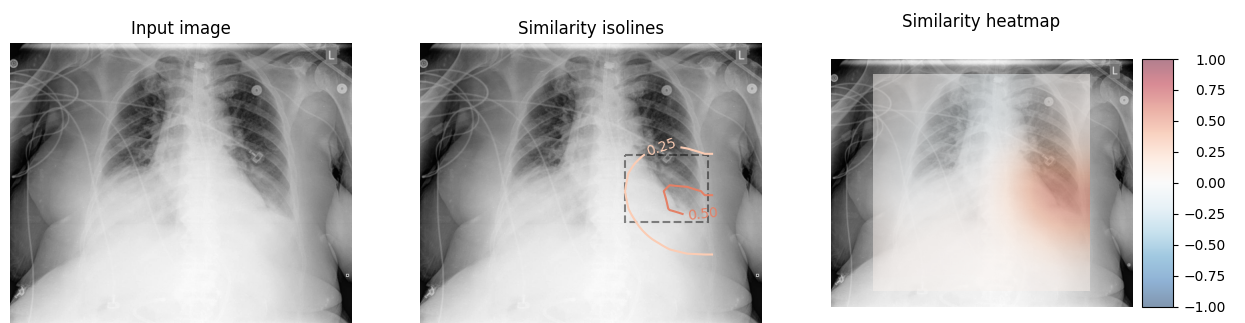
\includegraphics[width=\linewidth]{microsoft-ml-medical-imagery.png}
    \caption{The ground-truth bounding box annotation for the phrase Left basilar consolidation seen is shown in the middle figure (in black). Generated with HI-ML toolbox for deep learning for medical imaging and Azure integration}
    \label{fig:microsoft_medical_imagery}
\end{figure}

\subsubsection{Hallucination Mitigation in Medical MLLMs}
Hallucination mitigation is directly relevant to two ACE clinical actions: Diagnosis, where factually incorrect explanations can mislead clinical decisions, and Audit, where explanation traceability and grounding in real cases are regulatory requirements.
Multimodal Large Language Models suffer from hallucinations---generating plausible but incorrect medical information. Visual Retrieval-Augmented Generation (V-RAG) addresses this by retrieving similar images and reports to ground predictions \cite{chu2025reducinghallucinationsmedicalmultimodal}.

\textbf{V-RAG Framework:}
\begin{equation}
\mathcal{R}_k(x)=\operatorname{top\text{-}k}_{z \in \mathcal{D}} \cos \big(e(x), e(z)\big),
\label{eq:vrag_retrieval}
\end{equation}
In Equation~\eqref{eq:vrag_retrieval}, $e(\cdot)$ is a joint image-text encoder and $\mathcal{R}_k(x)$ returns the top-$k$ retrieved support cases.
\begin{itemize}
    \item Retrieves top-k similar images using embeddings from MedCLIP encoder
    \item Compares query image with retrieved images via cross-modal attention
    \item Uses entity probing to verify disease entities against knowledge base
    \item Employs LLM (Llama 3.1 70B) to rewrite reports based on verified entities
    \item Achieved 15-20\% improvement in RadGraph-F1 scores vs. baseline generation
\end{itemize}

This approach provides post-hoc explainability through retrieval citation, showing clinicians which cases informed the prediction \cite{chu2025reducinghallucinationsmedicalmultimodal}.
\begin{tcolorbox}[colback=green!5,colframe=green!50!black,title=\textbf{Clinical Suitability Assessment: Retrieval-Grounded Explanations}]
\textbf{Audit: Promising}. We evaluated a retrieval-only proxy rather than the full V-RAG stack: nearest-case retrieval added $2.35$ ms/case and achieved evidence purity $0.413$ on the spurious baseline, increasing to $0.584$ after causal training. \textbf{Diagnosis: Conditional}. Retrieval improves traceability, but our experiment does not measure report rewriting latency or citation hallucinations. \textbf{Key gap}: full V-RAG pipelines remain constrained by retrieval quality and downstream LLM latency.
\end{tcolorbox}
From an ACE perspective, retrieval-grounded explanations represent one of the most promising current approach for satisfying the auditability requirement, as they provide explicit evidence trails linking predictions to real clinical cases.

\subsubsection{Modality-Specific Explanations}

While MXAI methods often focus on integrating information across modalities, it's equally important to understand the contribution of each individual modality to the final prediction. Modality-specific explanations aim to answer the question: "How important was each modality for this prediction, and why?" This is particularly crucial in healthcare, where different modalities can provide complementary information, and understanding their individual roles can aid clinical decision-making.

\textbf{Methods for Modality-Specific Explanations:}

\begin{itemize}
    \item \textbf{Modality Ablation:} One approach is to systematically remove or perturb the information from each modality and observe the effect on the model's prediction. For example, one could mask out the image modality and see how the prediction changes when only text data is available. This can provide a direct measure of modality importance:
    \begin{equation}
    \Delta_m(x) = f(x) - f(x_{\setminus m}),
    \label{eq:modality_ablation}    
    \end{equation}
    In Equation~\eqref{eq:modality_ablation}, $x_{\setminus m}$ denotes the input with modality $m$ removed or replaced by a neutral baseline.
    \item \textbf{Modality-Specific Feature Importance:} Techniques like SHAP can be adapted to provide modality-specific feature importance scores. This involves calculating SHAP values for features within each modality separately, providing insights into which features within each modality are most influential.
    \item \textbf{Decomposed Attention:} In models with attention mechanisms, it's possible to decompose the attention weights to determine how much attention is being paid to each modality at different stages of processing. This can reveal which modality is driving the prediction at each step.
\end{itemize}

\begin{tcolorbox}[colback=green!5,colframe=green!50!black,title=\textbf{Clinical Suitability Assessment: Modality Ablation}]
\textbf{Treatment and Monitoring: Strong candidate}. Mean latency was $3.98$ ms/case with causal alignment $\rho=1.00$ and seed stability $0.827$ in our benchmark. On the OOD shift, masking the non-causal \textit{hospital\_bias} feature reduced baseline accuracy by $42.9$ points, directly exposing spurious multimodal dependence. \textbf{Audit: Partially suitable}. The mechanism is transparent, but interpretation still depends on the chosen masking intervention. \textbf{Key gap}: inter-modality dependencies can make single-modality removal overestimate importance.
\end{tcolorbox}

\textbf{Example in Healthcare:}

Consider an MXAI model used for diagnosing skin cancer from dermoscopic images and patient metadata (age, gender, lesion location). Modality-specific explanations could reveal that for a particular patient, the model heavily relied on the image modality due to the presence of specific visual features indicative of malignancy, while the metadata played a lesser role. This information can be crucial for clinicians in understanding the basis of the AI's diagnosis.

\textbf{Challenges:}

\begin{itemize}
    \item \textbf{Inter-Modality Dependencies:} 
    Disentangling modality contributions is particularly challenging when modalities carry overlapping information. This was directly observed in our controlled benchmark (Section 6): masking the spurious hospital feature caused a 51.7-point accuracy drop, nearly identical to masking the biomarker feature (50.8 points), suggesting that the model had learned a partially redundant representation across modalities that single-modality ablation alone cannot fully resolve.}
%it can be challenging to disentangle the contributions of different modalities when they are highly interdependent. For example, an image and its corresponding textual description may contain overlapping information.

    \item \textbf{Defining Modality Boundaries:} 
    The definition of intervention boundaries directly affects ablation results. In our benchmark, replacing the hospital token with a neutral baseline produced different importance rankings than full feature removal, confirming that the choice of masking strategy is not neutral and must be documented for clinical reproducibility.}
    %In some cases, the boundaries between modalities may not be clear-cut. For instance, should a clinical note be considered a single modality, or should it be further subdivided into sections like "patient history," "symptoms," and "lab results"?
\end{itemize}

\textbf{Future Directions:}
Research into modality-specific explanations should focus on developing methods that can handle complex inter-modality dependencies and provide more granular insights into the role of each modality. Combining modality-specific explanations with cross-modal attention mechanisms could offer a comprehensive understanding of how multimodal models make decisions. Furthermore, developing interactive visualization tools that allow clinicians to explore modality-specific contributions could enhance the usability of MXAI in healthcare \cite{holzinger2019causability}.

\subsection{MXAI Architectures}

This subsection outlines the key architectural designs for multimodal learning, focusing on how different modalities are integrated and processed within AI models.

Multimodal architectures are designed to process and integrate information from different data modalities. In healthcare, these architectures are essential for leveraging the diverse types of data available, such as medical images, clinical notes, and genomic data. Effective integration of these modalities can lead to more accurate and comprehensive diagnostic and prognostic models.


\textbf{Transformers and Attention Models:} 
    As introduced in subsection \ref{subsection:multimodalaiandxai}, transformers model cross-modal relationships through attention mechanisms, enabling effective integration of imaging and clinical data in healthcare \cite{rodis2024multimodalexplainableartificialintelligence, HOFMANN2022119504}
    %As discussed, transformers, particularly with their attention mechanisms, have become central to multimodal learning. They excel at modeling relationships between different modalities, making them suitable for tasks like visual question answering and multimodal machine translation. In healthcare, transformers can integrate and analyze data from various sources, such as combining imaging data with patient records to improve diagnostic accuracy \cite{rodis2024multimodalexplainableartificialintelligence, HOFMANN2022119504}. For example, a transformer model can analyze both MRI scans and clinical notes to provide a more holistic diagnosis of neurological conditions, leveraging the strengths of both modalities to enhance prediction reliability.
\textbf{Advanced Fusion Networks:} Recent architectures address modality dropout, missing data, and causal alignment through attention-based fusion. MDFormer focuses on robustness to missing modalities, while CausalCLIPSeg introduces causal intervention into CLIP-based medical segmentation \cite{li2025mdformer,chen2025causalclipsegunlockingclipspotential}.

\textbf{Neuro-Symbolic Integration:} Combining neural networks with medical ontologies or semantic layers can make explanations more rule-grounded and easier to audit in distributed healthcare settings. SemFedXAI is one example of this direction \cite{info16060435}.
    
    \textbf{Multimodal Fusion Strategies }

    Three main fusion strategies are compared in Figure \ref{fig:multimodal_fusion_strategies}.
\subsubsection{Early Fusion (Feature-Level Fusion)}
Early fusion involves combining the raw data or features from different modalities at an early stage of processing. This can be as simple as concatenating feature vectors from each modality before feeding them into a single model.
        
        \textbf{Example in Healthcare:} In early fusion, genomic data, clinical notes, and medical images can be processed by modality-specific encoders to extract relevant features. These features are then concatenated into a single feature vector and fed into a classifier for disease diagnosis. For instance, an early fusion model might combine features extracted from MRI scans, genomic sequences, and patient history to predict the likelihood of Alzheimer's disease.
        
        \textbf{Advantages:}
        \begin{itemize}
            \item Allows the model to learn interactions between modalities early on.
            \item Can potentially capture low-level correlations between modalities.
        \end{itemize}

        \textbf{Challenges:}
        \begin{itemize}
            \item May be difficult to align modalities with different structures and temporal resolutions.
            \item Can result in high-dimensional feature vectors, increasing computational complexity.
        \end{itemize}
        
       \subsubsection{Late Fusion (Decision-Level Fusion)} 
       Late fusion involves training separate models on each modality and then combining their predictions at a later stage. This can be done using techniques like averaging, voting, or stacking.
        
        \textbf{Example in Healthcare:} Separate models can be trained to analyze medical images, genomic data, and clinical notes independently. The predictions from each model are then combined using a fusion mechanism, such as a weighted average, to make the final diagnosis. For example, one model might predict the likelihood of cancer from a CT scan, another from genomic data, and a third from patient history. The final prediction is then made by combining the outputs of these models.
                
        \textbf{Advantages:}
        \begin{itemize}
            \item Easier to implement as it doesn't require joint training of modalities.
            \item Allows for the use of modality-specific models that are optimized for each data type.
        \end{itemize}

        \textbf{Challenges:}
        \begin{itemize}
            \item May not capture cross-modal interactions as effectively as early fusion.
            \item Requires careful calibration of the individual models to ensure their predictions are comparable.
        \end{itemize}

        \subsubsection{Hybrid Fusion} 
        Hybrid fusion combines aspects of both early and late fusion. For example, some modalities might be fused early on, while others are fused later, or intermediate representations from modality-specific models might be combined and processed jointly. Figure \ref{fig:multimodal_fusion_strategies} summarizes the three multimodal fusion strategies.
        
        \textbf{Example in Healthcare:} A hybrid fusion model might combine features from medical images and genomic data using early fusion, while incorporating clinical notes at a later stage through late fusion. This allows the model to learn interactions between images and genomic data early on, while also leveraging the predictions of a separate model trained on clinical notes. For instance, a hybrid model for predicting treatment response in cancer patients might use early fusion to combine features from PET scans and genomic profiles, and then use late fusion to integrate the predictions from a model trained on the patient's medical history and lab results.

        \textbf{Advantages:}
        \begin{itemize}
            \item Offers flexibility to choose the best fusion strategy for each modality.
            \item Can potentially capture both low-level and high-level interactions between modalities.
        \end{itemize}

        \textbf{Challenges:}
        \begin{itemize}
            \item More complex to design and implement than early or late fusion.
            \item Requires careful tuning of the fusion points and strategies.
        \end{itemize}
    
    \begin{figure}
        \centering
        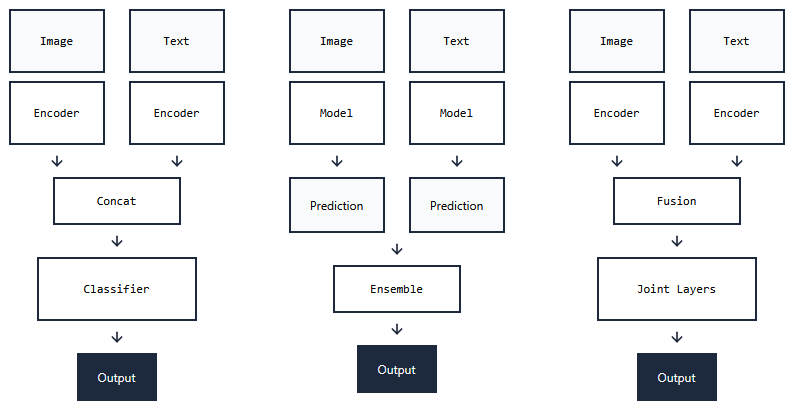
\includegraphics[width=\linewidth]{ml_pipeline.png}
        \caption{The current 3 multimodal fusion strategies}
        \label{fig:multimodal_fusion_strategies}
    \end{figure}

    \textbf{Applications in Healthcare:}
    Multimodal fusion has been successfully applied in various healthcare applications. For example, \cite{SUK2014569} developed a multimodal fusion model for early diagnosis of Alzheimer's disease, integrating MRI scans, PET scans, and cognitive test scores using a combination of early and late fusion. Their results illustrate the clinical value of combining complementary modalities for diagnostic support.

    \textbf{Future Directions:}
    Future research in multimodal fusion for MXAI should focus on developing more adaptive and dynamic fusion strategies that can automatically determine the optimal fusion points and methods based on the specific characteristics of the data and the task. Additionally, exploring how to explain the fusion process itself, i.e., understanding how the model combines information from different modalities, is a crucial area for future work in MXAI.

\textbf{Hybrid Models:} 
Hybrid models such as DeepXplainer \cite{wani2024deepxplainer} combine CNNs with tree-based classifiers to balance performance and interpretability, as discussed in Section 2.2.
    %These combine different model types to leverage their strengths. For example, DeepXplainer combines CNNs and tree-based models to improve both accuracy and explainability. In healthcare, hybrid models can offer the performance benefits of deep learning with the interpretability of simpler models. For instance, a hybrid model might use a CNN to process medical images and a decision tree to incorporate clinical data, providing both high accuracy and clear explanations for the predictions \cite{wani2024deepxplainer}. Combining the strengths of different model types helps in developing robust and interpretable AI systems for various healthcare applications.


\textbf{Conclusion of MXAI Architectures:}

The architectural designs for multimodal learning, including transformers, fusion networks, and hybrid models, play a crucial role in advancing MXAI in healthcare. These architectures enable the effective integration and processing of diverse data modalities, leading to improved diagnostic and prognostic models. However, the choice of architecture depends on the specific application and the nature of the data. Future research should focus on developing more sophisticated and efficient architectures that can handle the complexity and heterogeneity of healthcare data while maintaining interpretability.

\subsection{Applications of MXAI in Healthcare}

This subsection showcases how MXAI is being applied in various medical fields, highlighting specific examples and case studies.

Multimodal XAI has been successfully applied in diverse fields, demonstrating its versatility and impact. In healthcare, MXAI enhances diagnostic accuracy, personalizes treatment plans, and improves decision-making processes by integrating and interpreting data from multiple modalities. \textcolor{red}{Unless explicitly described as a reported deployment or clinical study, the workflows in this section are illustrative scenarios used to show how MXAI methods could support clinical actions. They should not be interpreted as evidence of clinical deployment or validated patient benefit. }

\subsubsection{Disease Diagnosis}

MXAI is used to improve diagnostic accuracy by integrating data from medical images, patient records, and lab results. Integrating multiple data sources allows for a more comprehensive understanding of a patient's condition, leading to more accurate diagnoses.
The following workflows are illustrative scenarios designed to exemplify how MXAI methods could be applied in clinical settings. They do not report empirical results from deployed systems unless explicitly referenced.


     \textbf{Cancer Diagnosis and Prognosis:} Models combining histopathological images with genomic data can aid in cancer diagnosis and prognosis. Explainable methods like Grad-CAM and SHAP are used to highlight the regions in images and the genomic features that contribute to the diagnosis. For example, combining image analysis of tumor biopsies with genomic data can provide insights into tumor heterogeneity and inform treatment decisions \cite{Mohan_2025, wani2024deepxplainer}.

    \textbf{Breast Cancer Diagnosis}
    \begin{itemize}
        \item \textbf{Medical Problem:} Accurate and early diagnosis of breast cancer is crucial for effective treatment and improved patient outcomes.
        \item \textbf{Modalities Used:} Mammograms (images) and patient clinical data (age, family history, etc.).
        \item \textbf{MXAI Methods Applied:} A combination of CNNs for image analysis and Random Forests for processing clinical data. Grad-CAM was used to highlight suspicious regions on mammograms, and SHAP values were used to explain the contribution of clinical factors.
        \item \textbf{Explanation Role:} This workflow illustrates how Grad-CAM and SHAP can jointly expose suspicious image regions and influential clinical covariates in breast-cancer screening pipelines \cite{Bai_2025}.
        \item \textbf{Potential Clinical Use:} In practice, such systems are best framed as reader-assistance tools that help contextualize predictions for radiologists rather than as standalone diagnostic replacements \cite{Bai_2025}.
    \end{itemize}

     \textbf{Neurological Disorders:} MXAI can integrate MRI scans, EEG data, and clinical notes to diagnose conditions like epilepsy and Alzheimer's disease. Attention mechanisms can highlight the brain regions and clinical factors contributing to the diagnosis, enhancing the interpretability of the model's predictions.
    
    \textbf{Alzheimer's Disease Diagnosis}
    \begin{itemize}
        \item \textbf{Medical Problem:} Early and accurate diagnosis of Alzheimer's disease is challenging but essential for timely intervention and management.
        \item \textbf{Modalities Used:} MRI scans, PET scans, cognitive test scores, and patient demographics.
        \item \textbf{MXAI Methods Applied:} A multimodal transformer model with cross-modal attention was used to integrate information from different modalities. Attention weights were visualized to show the relationships between brain regions in MRI/PET scans and cognitive scores.
        \item \textbf{Literature Anchor:} Multimodal fusion of MRI, PET, and cognitive scores has been reported for Alzheimer's diagnosis; the explanation workflow sketched here illustrates how cross-modal evidence could be surfaced to clinicians alongside such models \cite{SUK2014569}.
        \item \textbf{Potential Clinical Use:} The main value of this pattern is to summarize convergent evidence across modalities when early-stage findings are individually weak or noisy.
    \end{itemize}

     \textbf{Foundation Model Deployment Example: SimonMed-Lunit Partnership}
    \begin{itemize}
        \item \textbf{Medical Problem:} Scalable chest X-ray report generation across 175+ imaging centers
        \item \textbf{Modalities Used:} Chest X-rays (images) + Radiology reports (text)
        \item \textbf{MXAI Methods:} Lunit's CXR foundation model fine-tuned on SimonMed's data with attention-based cross-modal alignment; model cards provided for transparency
        \item \textbf{Publicly Reported Effect:} The deployment announcement describes faster report-generation workflows together with model monitoring for drift, but independent peer-reviewed validation remains limited \cite{lunit2025simonmed}
        \item \textbf{Why It Matters:} This example illustrates an industry pathway for operationalizing medical foundation models with monitoring hooks, even though it is not itself a full explainability evaluation \cite{lunit2025simonmed}
    \end{itemize}



\subsubsection{Treatment Planning}

MXAI can help personalize treatment plans by considering patient-specific multimodal data. Integrating data from various sources ensures that treatment plans are tailored to individual patient needs, improving treatment efficacy and patient outcomes.


    \textbf{Personalized Treatment Strategies:} Models integrating clinical notes, imaging data, and patient history can assist in determining optimal treatment strategies for complex diseases. For example, in oncology, MXAI can help tailor chemotherapy regimens based on tumor characteristics, patient genetics, and treatment response history.

     \textbf{Personalized Chemotherapy Regimens}
    \begin{itemize}
        \item \textbf{Medical Problem:} Determining the most effective chemotherapy regimen for individual cancer patients based on their unique characteristics and medical history.
        \item \textbf{Modalities Used:} Patient medical history (text), genomic data (tabular), and tumor images (images).
        \item \textbf{MXAI Methods Applied:} A hybrid fusion model combining a CNN for image analysis, an RNN for processing medical history, and a fully connected network for integrating genomic data. SHAP values were used to explain the contribution of each modality to the treatment recommendation.
        \item \textbf{Explanation Role:} This example illustrates how SHAP-style summaries can expose which genomic, imaging, and history features drive a treatment recommendation.
        \item \textbf{Potential Clinical Use:} The main promise is to support clinician review of personalized regimens by surfacing the multimodal factors behind the recommendation, not to replace oncology decision-making.
    \end{itemize}
    
     \textbf{Surgical Planning:} Transformer models have been employed to analyze laparoscopic videos, improving recognition and decision-making processes during surgeries \cite{rodis2024multimodalexplainableartificialintelligence}. Such models integrate text and image embeddings, enhancing prediction reliability and providing surgeons with valuable insights during procedures.For instance, a transformer model integrating chest X-rays with radiology reports can attend jointly to consolidation regions in the image and the phrase 'bilateral infiltrates' in the report, providing a grounded diagnostic explanation directly actionable by the radiologist.
    \textbf{Laparoscopic Surgery Assistance}
    \begin{itemize}
        \item \textbf{Medical Problem:} Enhancing the precision and safety of laparoscopic surgeries through real-time analysis and guidance.
        \item \textbf{Modalities Used:} Laparoscopic video feed (video) and surgical tool movement data (time-series).
        \item \textbf{MXAI Methods Applied:} A transformer-based model with attention mechanisms was used to analyze the video feed and tool movements. Attention maps highlighted critical anatomical structures and surgical actions.
        \item \textbf{Explanation Role:} The workflow illustrates how attention maps and temporal signals could support phase recognition and highlight potentially risky maneuvers in minimally invasive surgery \cite{SADEGHI2024109370}.
        \item \textbf{Potential Clinical Use:} The main near-term use is intraoperative decision support and surgical training, where explanations must remain low-latency and easy to inspect  \cite{SADEGHI2024109370}.
    \end{itemize}



\subsubsection{Case Studies}

Several case studies illustrate the successful application of MXAI in healthcare, demonstrating its potential to improve clinical practice.

\begin{itemize}
    \item \textbf{Lung Cancer Detection:} Sangeetha et al. (2024) developed a multimodal deep learning model for lung cancer detection that integrates genomic, clinical, and imaging data. The model uses a Multimodal Fusion Deep Neural Network (MFDNN) and provides explanations using SHAP values, highlighting the important features contributing to the prediction. This integration allows for early and accurate detection of lung cancer, improving patient prognosis \cite{wani2024deepxplainer}.
    \item \textbf{Skin Disease Classification:} Mohan et al. (2024) proposed an explainable deep learning framework for skin disease classification using Grad-CAM and SHAP. The framework provides visual explanations of the model's predictions, highlighting the regions in the images that are most relevant for the classification. This helps dermatologists understand and trust the AI's diagnostic decisions \cite{Mohan_2025}.
    \item \textbf{Surgical Video Analysis:} Abiyev et al. (2024) applied transformer models to analyze laparoscopic videos, improving the recognition of surgical phases and actions. The models integrate visual and textual information, and attention mechanisms are used to explain the model's predictions. This application enhances surgical training and can potentially improve surgical outcomes by providing real-time feedback and analysis \cite{rodis2024multimodalexplainableartificialintelligence}.
\end{itemize}

\textbf{Conclusion of Applications of MXAI in Healthcare:}
The applications reviewed in this section confirm that MXAI is actively deployed across diagnosis, treatment planning, and surgical assistance. However, when examined through the ACE framework, a consistent gap emerges: most systems optimize for explanation fidelity rather than for the specific properties (latency, causal validity, stability) required by the clinical action they target. Bridging this gap is the central challenge addressed in the remainder of this survey.
%MXAI has demonstrated significant potential in various healthcare applications, from disease diagnosis to treatment planning and surgical assistance. By integrating and interpreting multimodal data, MXAI models can provide more accurate, personalized, and interpretable insights, enhancing clinical decision-making and patient care. The case studies highlight the practical benefits of MXAI and underscore the importance of continued research and development in this area. Future work should focus on expanding the application of MXAI to other medical domains and addressing the challenges associated with its implementation in clinical practice.

\subsection{Comparative Analysis Revisited: Clinical Action Suitability}
%Traditional method comparison tables (ante-hoc vs. post-hoc, modality support) are replaced by Table \ref{tab:clinical_action_matrix}, which directly maps each method to its ability to support specific clinical decisions on the controlled benchmark. This matrix is the core evaluation tool for the empirical ACE framing used in this paper.
The proposed Clinical Action Suitability Matrix \ref{tab:clinical_action_matrix} constitutes a shift from conventional method-centric evaluations toward a clinically grounded, decision-oriented framework. Rather than categorizing methods along abstract technical dimensions (e.g., ante-hoc vs. post-hoc, modality compatibility), the matrix operationalizes explainability in terms of its ability to support concrete clinical actions under a controlled and reproducible benchmark. 

This reframing is motivated by a practical gap, clinicians and other domain experts must interpret and act upon model outputs without necessarily having the expertise to assess the underlying explainability methodology. 
As a result, the usefulness of an explanation is not determined solely by its theoretical guarantees, but by whether it provides clear, reliable, and timely support for a given decision. The matrix makes this connection explicit by translating technical properties (e.g., latency, stability, modality handling) into their implications for concrete clinical use.
By structuring the evaluation around actionability, the matrix aligns with an Action-Centered Explainability (ACE) perspective that emphasizes criteria that are directly relevant to end users, such as whether an explanation can be obtained within clinically acceptable time constraints, whether it remains consistent across model updates, and whether it provides sufficiently transparent reasoning to justify or audit a decision.

Another key contribution of this formulation is the explicit inclusion of failure modes and regulatory gaps alongside performance-related attributes. This acknowledges that, in clinical contexts, limitations such as sensitivity to spurious correlations, lack of uncertainty quantification, or absence of standardized protocols directly impact the safety and deployability of a method. As such, the matrix captures not only what methods can explain, but also under which conditions those explanations may become unreliable or non-compliant with the requirements.
While Table 2 (Section 3.3) summarizes measured benchmark results per method, Table 3 extends this evaluation by explicitly mapping technical properties to clinical deployment constraints and regulatory gaps.

\begin{landscape}
\begin{table}[p]
\centering
\caption{Controlled Clinical Action Suitability Matrix for MXAI Methods}
\label{tab:clinical_action_matrix}

\scriptsize
\setlength{\tabcolsep}{3pt}
\renewcommand{\arraystretch}{1.25}

\begin{tabularx}{\linewidth}{|L{2.2cm}|L{3.0cm}|L{1.3cm}|L{1.1cm}|L{1.6cm}|L{1.8cm}|Y|Y|Y|}
\hline
\textbf{Method} &
\textbf{Clinical Action} &
\textbf{Latency} &
\textbf{Causal?} &
\textbf{Stability} &
\textbf{Modality Support} &
\textbf{Advantages for Action} &
\textbf{Critical Failure Mode} &
\textbf{Regulatory Gap} \\
\hline

KernelSHAP &
\makecell[l]{Triage: \textcolor{red}{\xmark}\\
Diagnosis: \partialcmark\\
Treatment: \partialcmark\\
Audit: \partialcmark\\
Monitoring: \textcolor{red}{\xmark}} &
142.66 ms & No & 0.844 & Image + tabular (grouped) &
High retraining consistency &
Slow perturbational evaluation &
No audit trail or uncertainty bound \\
\hline

LIME &
\makecell[l]{Triage: \textcolor{red}{\xmark}\\
Diagnosis: \partialcmark\\
Treatment: \partialcmark\\
Audit: \partialcmark\\
Monitoring: \textcolor{red}{\xmark}} &
48.75 ms & No & 0.826 & Image + tabular (grouped) &
Interpretable local surrogate &
Neighborhood sensitivity &
No standardized perturbation policy \\
\hline

Integrated Gradients &
\makecell[l]{Triage: \partialcmark\\
Diagnosis: \partialcmark\\
Treatment: \textcolor{red}{\xmark}\\
Audit: \partialcmark\\
Monitoring: \textcolor{red}{\xmark}} &
5.62 ms & No & 0.875 & Differentiable multimodal models &
Fast gradient-based ranking &
Baseline dependence &
No explanation confidence estimate \\
\hline

Grad-CAM &
\makecell[l]{Triage: \textcolor{green}{\cmark}\\
Diagnosis: \partialcmark\\
Treatment: \textcolor{red}{\xmark}\\
Audit: \textcolor{red}{\xmark}\\
Monitoring: \textcolor{red}{\xmark}} &
2.30 ms & No & 0.868 & Image branch only &
Fastest visual localization &
Leakage score 0.056 under metadata shift &
No stability guarantee \\
\hline

Cross-Modal Attention &
\makecell[l]{Triage: \textcolor{green}{\cmark}\\
Diagnosis: \partialcmark\\
Treatment: \textcolor{red}{\xmark}\\
Audit: \partialcmark\\
Monitoring: \textcolor{red}{\xmark}} &
1.15 ms & No & 0.847 & Image + tabular tokens &
Fastest intrinsic explanation &
Highest mean weight on spurious hospital token &
No counterfactual validity or uncertainty \\
\hline

Retrieval Proxy &
\makecell[l]{Triage: \textcolor{green}{\cmark}\\
Diagnosis: \partialcmark\\
Treatment: \partialcmark\\
Audit: \textcolor{green}{\cmark}\\
Monitoring: \partialcmark} &
2.35 ms & Partial & Trace-based & Joint embedding retrieval &
Explicit evidence trail &
Evidence purity only 0.413 on spurious baseline &
0.584 after causal training \\
\hline

Modality Ablation &
\makecell[l]{Triage: \textcolor{green}{\cmark}\\
Diagnosis: \textcolor{green}{\cmark}\\
Treatment: \textcolor{green}{\cmark}\\
Audit: \partialcmark\\
Monitoring: \textcolor{green}{\cmark}} &
3.98 ms & Partial & 0.827 & Multimodal &
Direct intervention test &
Intervention definition matters &
No standardized masking protocol \\
\hline
\end{tabularx}

\vspace{4pt}
{\footnotesize\textit{Stability values are cosine similarity across retrained models. Green = suitable, Yellow = partially suitable, Red = unsuitable. Ratings follow the controlled benchmark rather than universal clinical claims.}}
\end{table}
\end{landscape}


\textbf{Key Insight:} 
No method satisfied all clinical actions simultaneously on the controlled benchmark highlighting a limitation of current explanation paradigms. 
The matrix shows that each explanation paradigm optimizes for a subset of clinically relevant properties, but none simultaneously achieves the latency constraints, stability requirements, and interventional validity needed across the full set of clinical actions.

%No method satisfied all clinical actions simultaneously on the controlled benchmark. 
%The dominant trade-off was between latency and intervention-faithfulness: intrinsic attention and Grad-CAM were fastest, whereas modality ablation was the strongest monitoring/treatment tool and perturbational explainers were much slower.

The dominant trade-off is between latency and interventional faithfulness. Methods that derive explanations directly from internal model computations, such as intrinsic attention and Grad-CAM, achieve very low latency and are well-suited for time-constrained settings like triage. However, their explanations remain correlational, reflecting internal model sensitivities rather than the effect of controlled input changes, which limits their reliability for decisions requiring causal reasoning.

In contrast, modality ablation approximates interventional reasoning by explicitly modifying inputs and observing prediction changes, making it more suitable for treatment and monitoring tasks. This improved faithfulness, however, comes with higher computational cost and sensitivity to how interventions are defined, affecting reproducibility. Perturbation-based methods such as KernelSHAP and LIME follow a similar logic at finer granularity, providing stable attributions but incurring substantial latency, which restricts their use to offline analysis or audit scenarios.

In summary, the controlled benchmark reveals a fundamental trade-off that no current method resolves: methods fast enough for real-time clinical use (attention, Grad-CAM) lack interventional guarantees, while those that approximate causal reasoning (KernelSHAP, modality ablation) are too slow or operationally sensitive for continuous deployment. ACE makes this trade-off explicit and actionable by mapping it to specific clinical actions rather than treating it as an abstract algorithmic limitation.

\begin{table}[h!]
\centering
\caption{Summary of Gaps and Recommendations for MXAI Methods Across Clinical Actions}
\begin{tabularx}{\linewidth}{|X|X|X|X|}
\hline
\textbf{Clinical Action} & \textbf{Promising Methods} & \textbf{Key Gaps} & \textbf{Recommendation / Usage} \\ \hline
Triage & Attention, Grad-CAM & Latency critical, limited causal validity & Use attention for real-time speed; combine with causal training if possible \\ \hline
Diagnosis & Integrated Gradients, KernelSHAP & Attention and Grad-CAM biased by non-causal features & Prioritize causal methods; verify cross-modal alignment \\ \hline
Treatment & Modality Ablation, SHAP & High computational cost; sensitive to intervention definition & Apply in batch pipelines; document masking/intervention choices \\ \hline
Audit & Retrieval-Grounded, KernelSHAP & Lack of standardization; no confidence intervals & Maintain explicit audit trails; combine with retrieval for traceability \\ \hline
Monitoring & Modality Ablation, Retrieval Proxy & Limited temporal stability for some methods & Add recalibration / drift detection; monitor OOD shifts \\ \hline
\end{tabularx}
\label{tab:mxai_gaps}
\end{table}

\noindent
\textit{Note:} This table summarizes the most suitable MXAI methods per clinical action, highlights observed limitations in controlled benchmarks, and provides practical guidance for deployment in healthcare settings.

\section{Datasets and Benchmarks}

This section discusses commonly used datasets for MXAI research in healthcare and the challenges of creating representative datasets. It also touches upon the need for standardized benchmarks to evaluate and compare MXAI methods.

\textcolor{red}{Datasets were selected when they satisfied at least one of three criteria: (i) they are widely used in multimodal medical AI/XAI research, (ii) they support evaluation of cross-modal reasoning or explanation fidelity, or (iii) they represent an ACE-relevant clinical action such as diagnosis, audit, or monitoring. This selection is not intended as an exhaustive catalogue of all medical datasets, but as a structured set of representative resources for evaluating action-centered MXAI.}

Datasets are crucial for training and evaluating multimodal AI models. Here are some commonly used datasets in MXAI research,  with a focus on healthcare applications:

Current datasets benchmark MXAI methods on proxy tasks (classification accuracy, captioning BLEU) that do not align with clinical actions. For example, VQA-Med evaluates explanation quality via answer correctness, not whether the explanation supports a treatment decision.\newline 
Future benchmarks must include action-specific metrics: latency distributions for triage, causal intervention accuracy for diagnosis, and explanation stability scores for audit trails, criteria operationalized in the controlled benchmark presented in Section 6 and the evaluation framework detailed in Section 7.

%Future benchmarks must include \textit{action-specific metrics}: latency distributions for triage, causal intervention accuracy for diagnosis, and explanation stability scores for audit trails.

\begin{itemize}
    \item \textbf{MIMIC-III (Medical Information Mart for Intensive Care III):} A large, publicly available database comprising de-identified health-related data associated with over forty thousand patients who stayed in critical care units. It includes various modalities such as clinical notes, vital signs, lab tests, and imaging reports. MIMIC-III is widely used for developing and evaluating predictive models for various clinical outcomes, such as mortality, length of stay, and readmission \cite{johnson2016mimic}.
    \item \textbf{VQA-Med:} A medical visual question answering dataset containing radiology images paired with questions and answers. It is used to evaluate models on their ability to understand and reason about medical images. VQA-Med challenges models to answer questions related to visual content in medical images, making it a valuable resource for developing and testing cross-modal attention mechanisms \cite{abacha2019vqa}.
    \item \textbf{HAM10000 (Human Against Machine with 10000 training images):} A dataset of 10,015 dermatoscopic images used for skin lesion classification. It is a valuable resource for training and evaluating models for skin cancer detection. HAM10000 provides a diverse set of skin lesion images, enabling the development of robust and generalizable models for dermatology \cite{Tschandl_2018}.
    \item \textbf{Cholec80:} A dataset of 80 cholecystectomy surgeries, annotated with phase and tool presence information. It is used for surgical video analysis and activity recognition. Cholec80 is crucial for developing AI systems that can understand and assist in surgical procedures, providing a rich source of multimodal data from real surgical settings \cite{twinanda2016endonetdeeparchitecturerecognition}.
    \item \textbf{LIDC-IDRI (Lung Image Database Consortium and Image Database Resource Initiative):} A dataset of thoracic computed tomography (CT) scans with annotations from multiple radiologists. It is widely used for lung cancer detection and segmentation. LIDC-IDRI provides detailed annotations that are essential for training models to accurately identify and segment lung nodules, contributing to early lung cancer detection \cite{armato2011lung}.
    \item \textbf{IU X-Ray:} This dataset contains 7,470 chest X-ray images and 3,955 associated radiology reports, collected from Indiana University hospitals. Each report includes sections for findings, impressions, and indications, providing a rich source of textual data linked to specific images. The dataset is used for tasks such as automated report generation and cross-modal retrieval, where models learn to associate specific findings in the reports with corresponding regions in the X-ray images. It's particularly valuable for developing and evaluating MXAI systems that integrate image and text data for improved diagnostic accuracy and explainability \cite{demner2016preparing}.
    \textcolor{re}{
    \item \textbf{SMMILE} is an expert-curated benchmark of 1,200 clinical problems designed to evaluate multimodal foundation models on few-shot in-context learning tasks, with multi-institutional radiologist review. It is particularly relevant for ACE's diagnosis and audit actions. PairDx contains 22,665 image-text pairs covering a broad range of medical conditions, designed for universal medical diagnosis evaluation across modalities.}
\end{itemize}

Table \ref{tab:datasets} summarizes commonly used datasets in MXAI research.

\begin{table}[h!]
\centering
\caption{Commonly Used Datasets for Multimodal XAI Research in Healthcare}
\begin{tabular}{|l|L{2cm}|L{3cm}|L{2.7cm}|L{2.5cm}|}
\hline
Dataset & Modality & Application & Size & Primary ACE Action \\ \hline
MIMIC-III & Text, Tabular, Image & Healthcare Analytics & Over 40,000 patients & Audit, Monitoring\\ \hline
VQA-Med & Text, Image & Visual Question Answering & Over 4,000 images & Diagnosis \\ \hline
HAM10000 & Image & Skin Disease Classification & 10,015 images & Diagnosis, Triage\\ \hline
Cholec80 & Video, Text & Surgical Video Analysis & 80 videos & Treatment selection \\ \hline 
LIDC-IDRI & CT Images & Lung Cancer Detection & 1,018 cases & Diagnosis, Triage\\ \hline
IU X-Ray & Text, Image & Automated Report Generation & 7,470 images, 3,955 reports & Diagnosis, Audit \\ \hline 
SMMILE & Image, Text & In-context learning evaluation & 1,200 clinical problems & Diagnosis, Audit\\ \hline
PairDx & Image, Text & Universal medical diagnosis & 22,665 image-text pairs & Diagnosis\\ 


\hline
\end{tabular}
\label{tab:datasets}
\end{table}

\subsection{Challenges in Dataset Creation and Benchmarking}

\begin{itemize}
    \item \textbf{Data Availability and Privacy:} In many domains, particularly healthcare, obtaining large, diverse, and well-annotated multimodal datasets is challenging due to data privacy concerns and the cost of data collection and annotation. Ensuring patient privacy while creating comprehensive datasets is a major hurdle.
    \item \textbf{Data Bias:} Datasets may be biased due to factors such as patient demographics, data collection procedures, and annotation practices. These biases can lead to models that perform poorly on underrepresented groups or in different settings. Addressing bias is crucial for developing fair and equitable MXAI systems.
    \item \textbf{Data Standardization:} Lack of standardization in data formats and annotation protocols can make it difficult to combine and compare datasets from different sources. Establishing common standards is essential for advancing MXAI research.
    \item \textbf{Multimodal Alignment:} Aligning data from different modalities can be challenging, particularly when the modalities are sampled at different rates or have different levels of granularity. Accurate alignment is crucial for training effective multimodal models.
\end{itemize}

\subsection{Benchmarks and Standardization Efforts}

Benchmarks are essential for evaluating and comparing the performance of different MXAI methods. They typically consist of a dataset, a set of tasks, and evaluation metrics. Several efforts are underway to establish standardized benchmarks for MXAI:


\textbf{ImageCLEF:} An annual evaluation campaign that includes tasks involving medical image analysis. The 2023 edition featured a task on visual question answering and generation in the medical domain, providing a benchmark for evaluating cross-modal understanding in MXAI systems \cite{crowe2023imageclef}.\\
\textbf{PhysioNet Challenges:} A series of challenges focused on physiological data, often including multiple modalities such as ECG, EEG, and other time-series data. These challenges provide benchmarks for tasks like arrhythmia detection and sleep stage classification \cite{goldberger2000physiobank}.\\
Despite these efforts, no existing benchmark simultaneously evaluates explanation latency, causal alignment, and stability under distribution shift, the three properties most critical under the ACE framework. The controlled benchmark introduced in Section 6 addresses this gap on a reproducible small-scale setting, while Section 7 proposes a broader evaluation protocol for future large-scale benchmarks.}\newline
\textbf{Conclusion of Datasets and Benchmarks:}

Datasets and benchmarks play a critical role in the development and evaluation of MXAI systems. While several valuable datasets exist, challenges related to data availability, privacy, bias, standardization, and alignment need to be addressed. Ongoing efforts to establish standardized benchmarks are crucial for advancing the field and ensuring the development of robust and reliable MXAI systems for healthcare. Future work should focus on creating more diverse and representative datasets, developing methods for aligning multimodal data, and establishing comprehensive benchmarks that cover a wide range of healthcare applications.


\section{Controlled Experimental Assessment of ACE Claims}
\label{sec:controlled_experiments}

To move several ACE assessments from literature-grounded judgment to measured evidence, we implemented a small but fully reproducible multimodal benchmark in the public github workspace. The goal was not to reproduce a hospital-scale deployment, but to stress the core claims that underlie the ACE taxonomy: explanation latency, robustness to spurious multimodal cues, stability across retraining, and cross-modal leakage.

\textcolor{red}{All benchmark scripts, raw predictions, summary tables, figure-generation code, seeds, and environment specifications are released in a public GitHub repository and archived on Zenodo. The expanded Section 6 benchmark uses 20 random seeds, a nine-value λ grid, 500 OOD cases, and 5000 bootstrap repetitions. The archive reports package versions, hardware details, and raw case-level predictions to support exact reproduction of the McNemar, Wilcoxon, and confidence-interval analyses. }

\subsection{Benchmark Design}

We used DermaMNIST, a $28 \times 28$ dermoscopic derivative of HAM10000 \cite{Tschandl_2018}, and augmented each image with four numeric clinical covariates: a moderately informative biomarker score, a moderately informative age-risk score, a strongly spurious hospital feature, and an uninformative administrative noise variable. The hospital feature was predictive during training but randomized at test time, creating a controlled out-of-distribution shift that separates correlation from causal usefulness.

The fusion model used a three-layer CNN image encoder, tokenized tabular inputs, and a single four-head self-attention block. We compared a standard model with a causal-invariance variant trained with
\begin{equation}
\mathcal{L}_{\text{total}} = \mathcal{L}_{\text{CE}}(f(x,z), y) + \lambda \left\| \sigma(f(x,z)) - \sigma(f(x,\tilde{z}_{\text{hospital}})) \right\|_2^2,
\label{eq:causal_invariance_objective}
\end{equation}

\textcolor{red}{In Equation~\eqref{eq:causal_invariance_objective}, $\tilde{z}_{\text{hospital}}$ permutes the hospital-bias feature within the batch. We trained each model on 2,000 samples for four epochs on an RTX 4050 Laptop GPU. To strengthen the robustness analysis, we evaluated model performance on a 500-case OOD subset across 20 random seeds and swept the causal-invariance weight $\lambda$ over nine values: $\{0.10, 0.25, 0.50, 0.75, 1.00, 1.50, 2.00, 3.00, 4.00\}$. Confidence intervals were estimated with 5,000 bootstrap resamples. Paired model comparisons used exact McNemar tests on pooled case-level correctness and Wilcoxon signed-rank tests across seeds.}

\textcolor{red}{We measured explanations on the same 500-case OOD subset using Captum implementations of attention extraction, Integrated Gradients, LIME, KernelSHAP, modality ablation, and Grad-CAM. Because the benchmark uses lightweight $28 \times 28$ images and a compact fusion backbone, absolute latencies should be interpreted as lower bounds relative to full-resolution clinical pipelines.}

\textcolor{red}{We also evaluated a retrieval-only case-based explainer as a lightweight proxy for retrieval-grounded explanation. Embeddings were extracted from the image encoder of the trained fusion model. For each OOD test case, the top-5 nearest training cases were retrieved by cosine similarity in embedding space. Evidence purity was measured as the proportion of retrieved cases sharing the ground-truth label with the query.}
%We also evaluated a retrieval-only case-based explainer as a lightweight proxy for retrieval-grounded explanation, measuring top-5 evidence purity and lookup latency without adding an LLM report-generation stage.
\subsection{Main Findings}
We first assess model-level robustness under the spurious shift (Table 5), then examine how this shift propagates into explanation behavior across methods (Table 6). The two tables should be read jointly: a model that relies on spurious features will produce explanations that reflect that reliance, regardless of the explainer used.

\begin{table}[h!]
\centering
\caption{Controlled robustness results under distribution shift.}
\label{tab:controlled_robustness}
\begin{tabular}{llllll}
\hline
\multicolumn{1}{|l|}{Model} &
\multicolumn{1}{l|}{$\lambda$} &
\multicolumn{1}{l|}{ID Acc.} &
\multicolumn{1}{l|}{OOD Acc. 500 \textcolor{red}{subset}} &
\multicolumn{1}{l|}{95\% Bootstrap CI} &
\multicolumn{1}{l|}{Generalization Gap} \\ \hline
\multicolumn{1}{|l|}{Baseline} &
\multicolumn{1}{l|}{0.00} &
\multicolumn{1}{l|}{0.854} &
\multicolumn{1}{l|}{0.604} &
\multicolumn{1}{l|}{{[}0.549, 0.662{]}} &
\multicolumn{1}{l|}{0.252} \\ \hline
\multicolumn{1}{|l|}{Causal invariance} &
\multicolumn{1}{l|}{4.00} &
\multicolumn{1}{l|}{0.843} &
\multicolumn{1}{l|}{0.753} &
\multicolumn{1}{l|}{{[}0.723, 0.777{]}} &
\multicolumn{1}{l|}{0.091} \\ \hline
\end{tabular}

\vspace{4pt}
{\footnotesize\textit{Generalization gaps are computed against the full OOD test split; bootstrap confidence intervals are estimated on the 500-case OOD evaluation subset.}}
\end{table}

\textcolor{red}{Table \ref{tab:controlled_robustness} shows that causal-invariance training improved mean OOD accuracy from 0.604 to 0.753, a 14.9-point gain on the 500-case OOD subset. The mean generalization gap decreased from 0.252 to 0.091, while in-distribution accuracy changed from 0.854 to 0.843, corresponding to a 1.1-point ID accuracy cost.} This directly supports the ACE claim that explanation quality must be evaluated jointly with intervention robustness, not only in-distribution fidelity. Figure \ref{fig:ace_benchmark_overview} provides an overview of the benchmark and its main performance/latency contrasts.

\begin{figure}[h!]
    \centering
    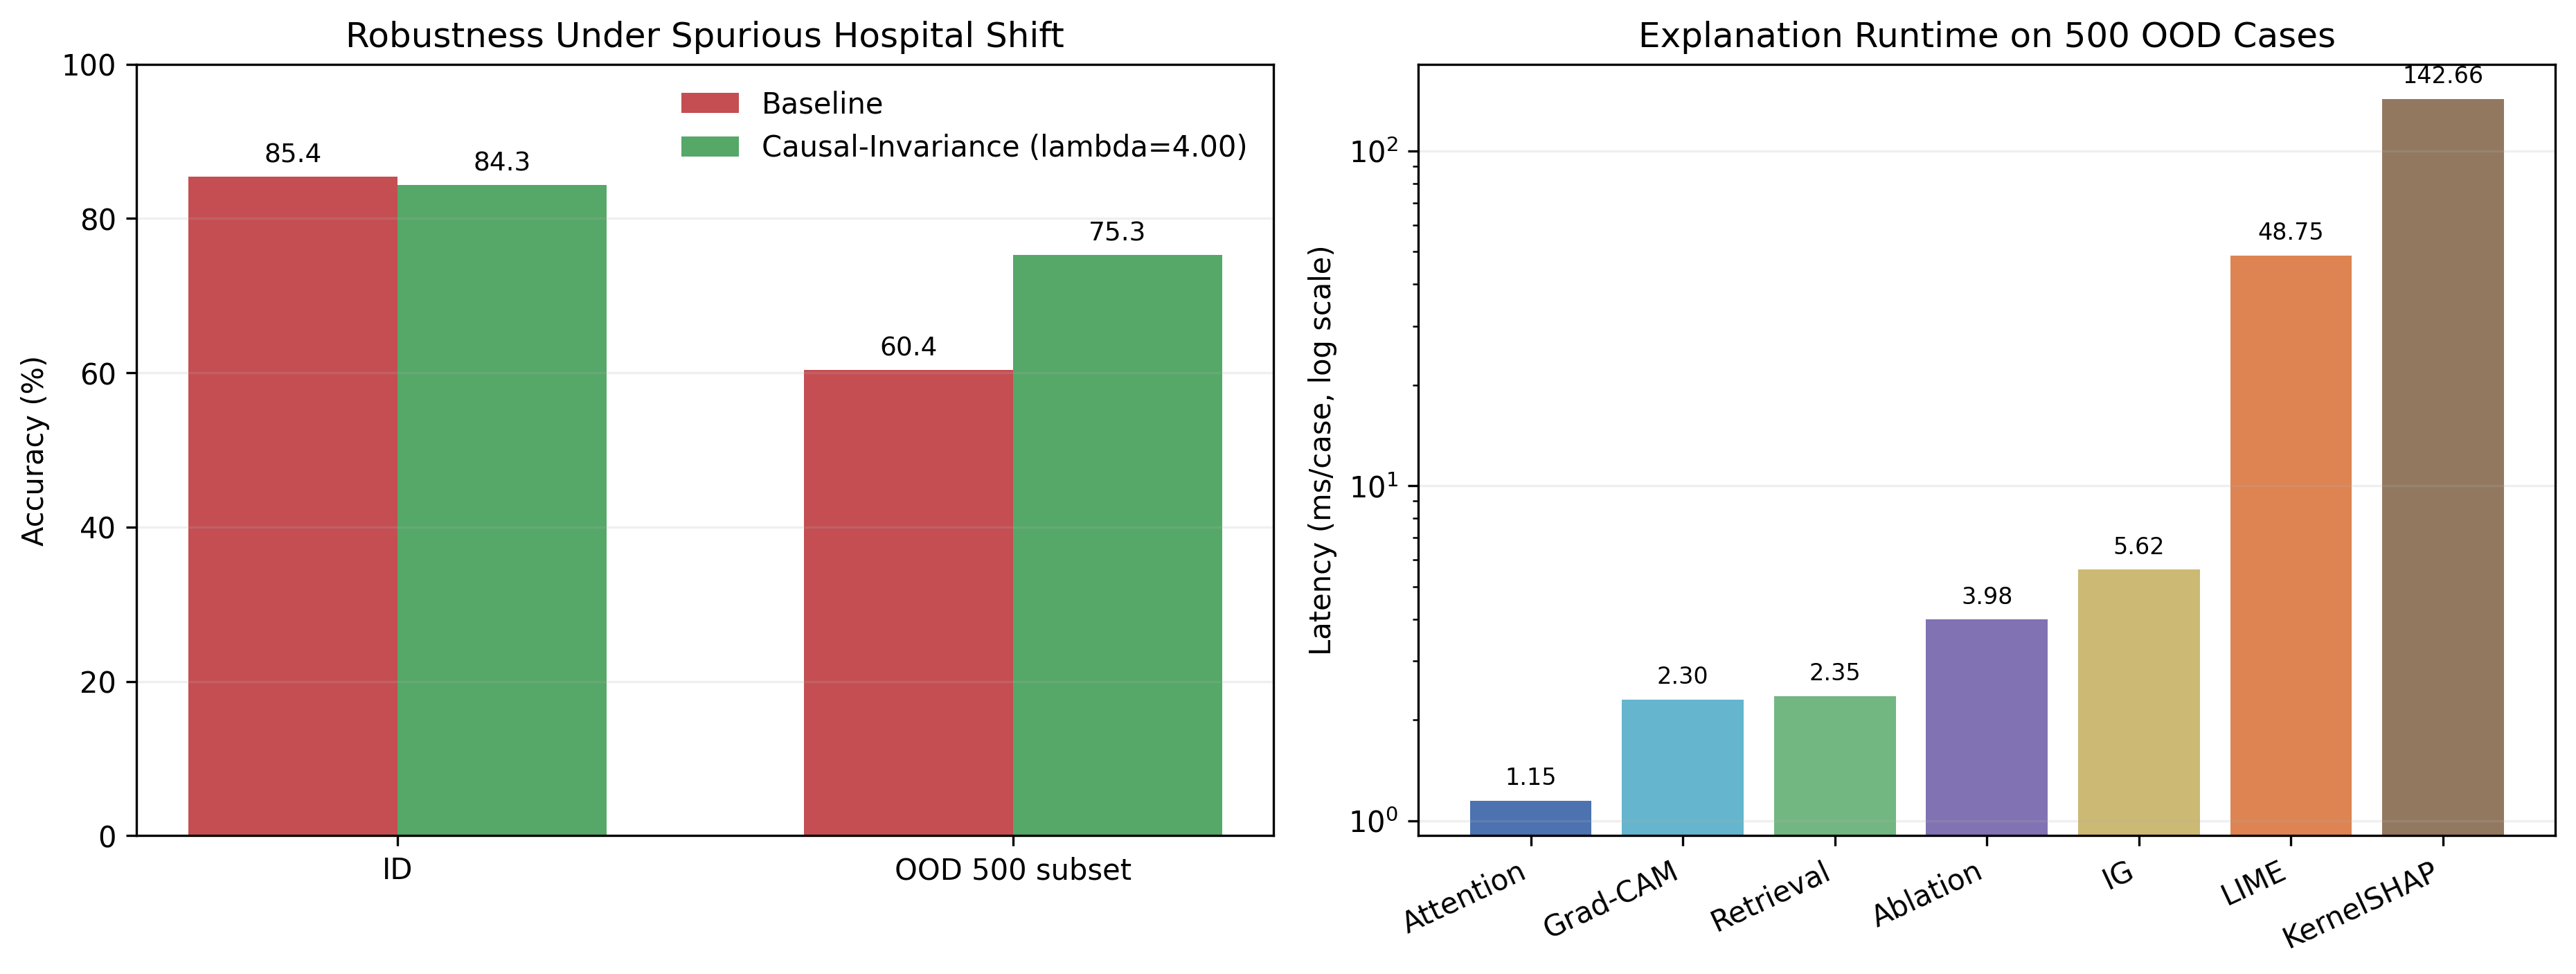
\includegraphics[width=\linewidth]{ace_benchmark_overview.png}
    \caption{Controlled benchmark overview. Left: baseline vs causal-invariance performance under the spurious hospital-feature shift. Right: explanation latency on the baseline model, showing the gap between intrinsic methods and perturbational explainers.}
    \label{fig:ace_benchmark_overview}
\end{figure}

\begin{table}[h!]
\centering
\caption{Measured explanation properties on the baseline model (500 OOD cases)}
\label{tab:controlled_methods}
{\scriptsize
\setlength{\tabcolsep}{4pt}
\renewcommand{\arraystretch}{1.15}
\begin{tabularx}{\textwidth}{|L{3.0cm}|Y|Y|Y|Y|}
\hline
\textbf{Method} & \textbf{Latency (ms/case)} & \textbf{Seed Stability} & \textbf{Causal Alignment} & \textbf{Grad-CAM Leakage} \\ \hline
Attention & 1.15 & 0.847 & 0.900 & -- \\ \hline
Integrated Gradients & 5.62 & 0.875 & 1.000 & -- \\ \hline
LIME & 48.75 & 0.826 & 0.900 & -- \\ \hline
KernelSHAP & 142.66 & 0.844 & 1.000 & -- \\ \hline
Modality ablation & 3.98 & 0.827 & 1.000 & -- \\ \hline
Grad-CAM & 2.30 & 0.868 & -- & 0.056 \\ \hline
Retrieval proxy & 2.35 & -- & -- & -- \\ \hline
\end{tabularx}
\par}
\vspace{4pt}
{\footnotesize\textit{Seed stability is cosine similarity across retrained models of the same variant. Causal alignment is the Spearman correlation between mean attribution ranking and accuracy drop under OOD feature masking. Grad-CAM leakage measures metadata-induced heatmap shift after perturbing only the tabular hospital-bias feature.}}
\end{table}


These measurements in Table \ref{tab:controlled_methods} partly confirm and partly refine the survey's qualitative assessments. Attention and Grad-CAM were indeed extremely fast, but Grad-CAM was the least stable method and the only one with clear cross-modal leakage under metadata-only perturbation. KernelSHAP and LIME were respectively about 124$\times$ and 42$\times$ slower than attention on the same model, validating their poor suitability for tight interaction loops even before scaling to larger clinical backbones. \newline
These latency figures are lower bounds measured on a lightweight 28×28 architecture; absolute runtimes will scale substantially with image resolution and model depth in real clinical pipelines.
At the same time, the controlled benchmark showed that ``post-hoc instability'' is not universal: LIME, KernelSHAP, and Integrated Gradients all reached seed stability above 0.82 on this lightweight architecture. The stronger empirical issue in our setting was spurious multimodal reliance. In the baseline model, the hospital feature masking caused an OOD accuracy drop of 0.429, and the mean attention weight on the hospital token exceeded the biomarker token. With the final causal-invariance weight ($\lambda=4.00$), hospital-feature reliance decreased from 0.429 to 0.279, hospital-token attention decreased from 0.410 to 0.265, Grad-CAM metadata leakage decreased from 0.056 to 0.016, and retrieval evidence purity increased from 0.413 to 0.584. This supports ACE's core argument: action-centered MXAI should prioritize intervention-aware validation, not explanation generation alone.

\begin{figure}[h!]
    \centering
    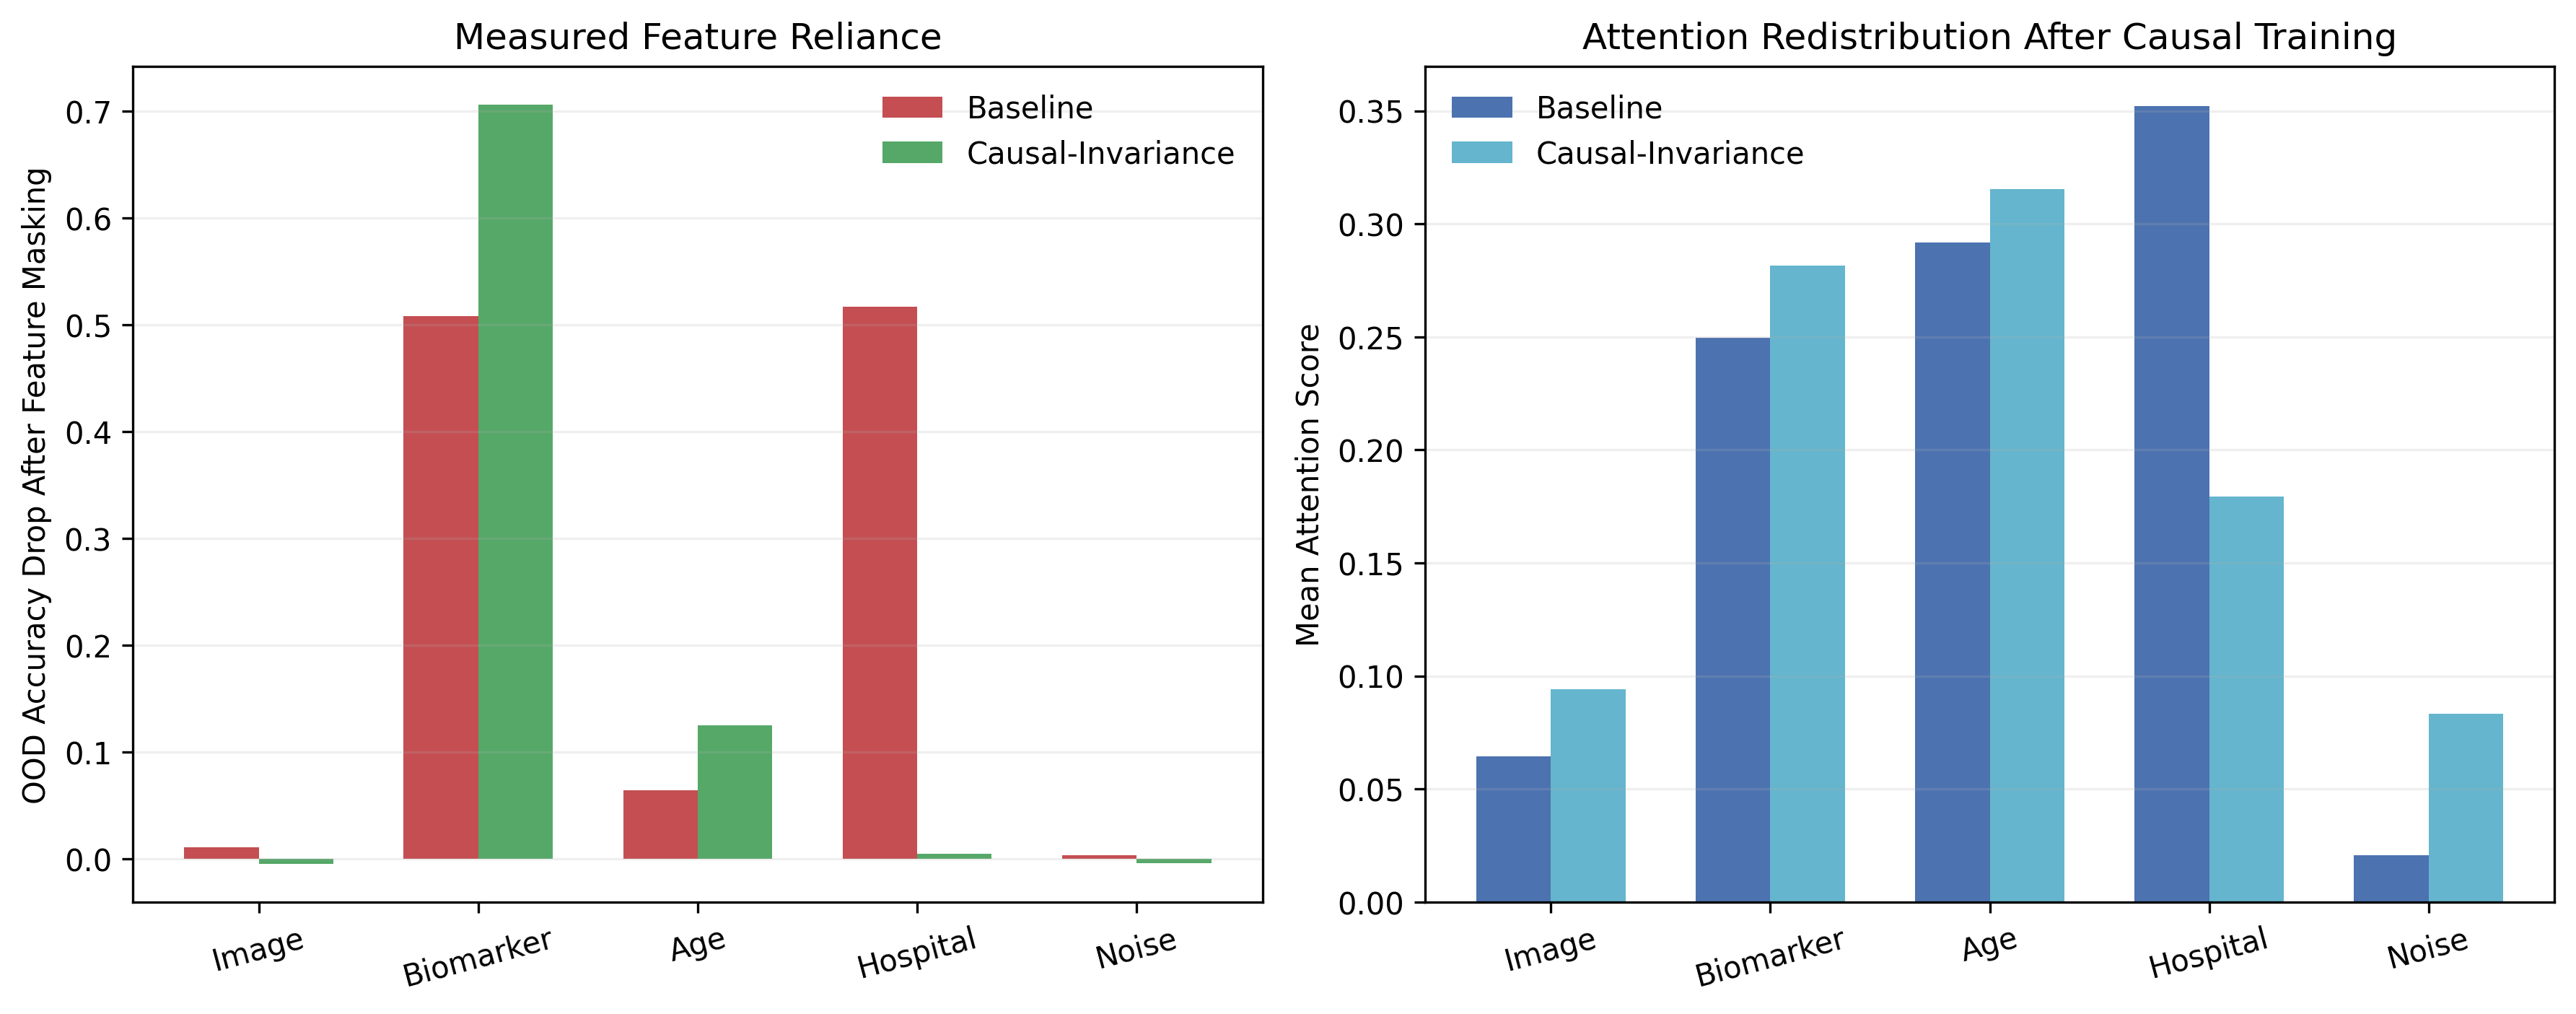
\includegraphics[width=\linewidth]{ace_spurious_signal.png}
    \caption{Effect of causal training on spurious multimodal reliance. Left: accuracy drop after feature masking on the OOD split. Right: mean attention redistribution from the non-causal hospital token toward clinically meaningful covariates.}
    \label{fig:ace_spurious_signal}
\end{figure}
Figure \ref{fig:ace_spurious_signal} shows two complementary effects of causal training. On the left, feature masking reveals that hospital-feature reliance drops from 0.429 to 0.279 after causal training, while clinically meaningful covariates remain influential. On the right, attention redistribution shows that the hospital token weight drops from 0.410 to 0.265, while image and biomarker tokens gain relative weight, visualizing improved explanation alignment alongside model robustness.
\section{Evaluation Metrics and Benchmarks}

Evaluation is the bottleneck of clinically viable MXAI. In healthcare, an explanation may appear faithful under standard proxy metrics while still failing to support diagnosis, misrepresenting cross-modal evidence, or breaking under distribution shift and model updates. For this reason, recent work has moved beyond purely technical XAI scores toward clinician-centered, multimodal, and regulatory evaluation criteria. This section organizes those criteria and shows how they align with the action-centered view proposed in this survey. Table \ref{tab:evaluation_frameworks} situates these requirements alongside recent clinical, multimodal, and causal evaluation frameworks for MXAI.

\subsection{Clinical-Centric Evaluation}

\textbf{Human-Centered Evaluation (HCE):} Stanford's HCE framework \cite{gambetti2025surveyhumancenteredevaluationexplainable} assesses:
\begin{itemize}
    \item \textbf{Cognitive Load:} Do explanations reduce or increase clinician mental effort?
    \item \textbf{Knowledge Alignment:} Do explanations match clinical reasoning patterns?
    \item \textbf{Trust Calibration:} Do explanations appropriately modulate clinician trust?
\end{itemize}

Within the ACE framework, human-centered evaluation dimensions can be interpreted as action-dependent requirements rather than generic usability criteria. Cognitive load is especially critical for triage and intra-operative assistance, where explanations must be rapidly interpretable under time pressure; knowledge alignment is central to diagnosis and treatment selection, where explanations should correspond to recognizable clinical reasoning patterns; and trust calibration is particularly important for audit and monitoring, where explanations must remain stable, defensible, and appropriately uncertain across model updates and deployment conditions.

\textbf{SMMILE Benchmark:} SMMILE \cite{rieff2025smmileexpertdrivenbenchmarkmultimodal} evaluates foundation models on few-shot clinical tasks with expert-curated cases and reports a substantial remaining gap between current MLLMs and expert human performance on complex reasoning tasks.

\subsection{Multimodal Explanation Metrics}

\textbf{Modality-Specific Feature Importance (MSFI):} Jin et al. \cite{Jin_2022} evaluated multiple heatmap algorithms against clinician-oriented requirements on multimodal medical images and reported substantial mismatch between highlighted regions and actual model decision logic.

\textbf{Cross-Modal Fidelity:} Measures explanation consistency when perturbing one modality and observing impact on explanations for others. RSA (2024) uses Representational Dissimilarity Matrices to assess explanation stability across model variants \cite{Sharma2025viz}.

Under ACE, cross-modal fidelity is especially important for diagnosis, where explanations should separate image-based evidence from metadata-driven shortcuts. We operationalize this failure mode as metadata-induced Grad-CAM shift: changes in the visual heatmap after perturbing only the tabular hospital-bias feature indicate cross-modal attribution leakage, reported in Table \ref{tab:controlled_methods}

\subsection{Regulatory Compliance Metrics}

FDA's 2025 draft guidance highlights the need for \cite{fda2025draft}:
\begin{itemize}
    \item \textbf{Explainability Validation:} User studies demonstrating clinicians can understand AI outputs
    \item \textbf{Bias Documentation:} Performance across demographic subgroups with correction plans
    \item \textbf{Uncertainty Quantification:} Confidence intervals for predictions with failure mode identification
\end{itemize}

\begin{table}[h!]
\centering
\caption{Operationalizing FDA-Oriented Requirements for MXAI Evaluation}
\label{tab:fda_operational_metrics}
{\scriptsize
\setlength{\tabcolsep}{3pt}
\renewcommand{\arraystretch}{1.2}
\begin{tabularx}{\textwidth}{|L{2.0cm}|L{2.5cm}|L{3.0cm}|L{3.0cm}|X|}
\hline
\textbf{FDA-Oriented Requirement} &
\textbf{MXAI Evaluation Question} &
\textbf{Operational Metric} &
\textbf{Suggested Reporting Threshold} &
\textbf{\textcolor{red}{ACE-Relevant Action}} \\ \hline

Explainability validation &
Can clinicians correctly interpret and use the explanation? &
Clinician comprehension score, decision-change rate, time-to-interpretation, explanation usefulness rating &
Report median and IQR; predefine task-specific non-inferiority criteria against standard clinical review &
\textcolor{red}{Triage, Diagnosis, Treatment selection} \\ \hline

Bias documentation &
Does the explanation remain reliable across patient subgroups and acquisition sites? &
Subgroup explanation stability, subgroup fidelity gap, demographic performance gap, site-specific attribution shift &
Report subgroup gaps with confidence intervals; flag clinically meaningful disparities across protected groups or acquisition sites &
\textcolor{red}{Diagnosis, Audit, Monitoring} \\ \hline

Uncertainty quantification &
Does the system indicate when its prediction or explanation may be unreliable? &
Prediction calibration error, explanation confidence interval, attribution variance across seeds or perturbations, abstention rate under uncertainty &
Report 95\% confidence intervals; define abstention or escalation rules for high-uncertainty cases &
\textcolor{red}{Triage, Audit, Monitoring} \\ \hline

Lifecycle monitoring &
Does explanation behavior remain stable after deployment or model updates? &
Update-to-update explanation drift, temporal attribution shift, OOD-trigger rate, recalibration frequency &
Predefine drift thresholds and revalidation triggers; report update-to-update explanation change before redeployment &
\textcolor{red}{Audit, Monitoring} \\ \hline

Traceability and documentation &
Can the explanation be reproduced and defended after the decision? &
Stored explanation record, model version, input provenance, retrieval evidence log, explanation-generation parameters &
Require versioned logs for all audited cases; record model version, input hash, seed, explainer parameters, and evidence sources &
\textcolor{red}{Audit} \\ \hline

Fairness of explanations &
Are equivalent clinical findings explained consistently across demographic groups and sites? &
Subgroup attribution agreement, subgroup causal-alignment gap, explanation calibration gap, subgroup leakage shift &
Report explanation-level fairness metrics by subgroup; investigate unexplained attribution gaps before clinical deployment &
\textcolor{red}{Triage, Diagnosis, Treatment selection, Audit, Monitoring} \\ \hline

\end{tabularx}
\par}
\end{table}

Table~\ref{tab:fda_operational_metrics} translates FDA-oriented transparency, bias, uncertainty, lifecycle, and documentation requirements into operational metrics that can be incorporated into MXAI evaluation pipelines.
These metrics are not currently reported in standard MXAI evaluations but are directly measurable within the ACE benchmark framework introduced in Section 6.
\textcolor{red}{Fairness should be evaluated not only at the predictive level but also at the explanation level: the same clinical evidence should not receive systematically different attribution across demographic groups, acquisition sites, or protected subgroups without clinical justification. }

\begin{table}[h!]
\centering
\caption{Modern Evaluation Frameworks for MXAI in Healthcare}
{\scriptsize
\setlength{\tabcolsep}{3pt}
\renewcommand{\arraystretch}{1.15}
\begin{tabularx}{\textwidth}{|L{2.4cm}|L{3.0cm}|L{4.0cm}|X|}
\hline
\textbf{Framework} & \textbf{Focus} & \textbf{Key Innovation} & \textbf{Clinical Validation} \\ \hline
SMMILE \cite{rieff2025smmileexpertdrivenbenchmarkmultimodal} & In-context learning & Expert-curated few-shot tasks & Multi-institutional radiologist review \\ \hline
HCE \cite{gambetti2025surveyhumancenteredevaluationexplainable} & Human-centered & Socio-technical gap analysis & workflow integration studies \\ \hline
MSFI \cite{Jin_2022} & Modality-specific & Clinical requirement grounding & 16 XAI algorithm failure analysis \\ \hline
MuCR \cite{li2025multimodalcausalreasoningbenchmark} & Causal reasoning & Cross-modal causality assessment & 12k causal image pairs \\ \hline
\end{tabularx}
\par}
\label{tab:evaluation_frameworks}
\end{table}

\subsection{ACE Cross-Dataset Stress-Test Benchmark}
\label{sec:ace_cross_dataset_suite}

To complement the single-domain proof-of-concept from Section \ref{sec:controlled_experiments}, we ran the same ACE evaluation pipeline on six public MedMNIST derivatives spanning hematology, dermatology, retinal OCT, abdominal CT, histopathology, and chest X-ray screening as described in \ref{tab:ace_suite_domains}. Each dataset was recast as a controlled multimodal task by pairing the image with the same four synthetic clinical covariates used in Section \ref{sec:controlled_experiments}, including a deliberately spurious hospital feature that was correlated with the label during training and randomized at test time. This cross-dataset suite was implemented in the public reproducibility repository \url{https://github.com/MathieuR-L/action-centered-XAI}, trained the same multimodal fusion backbone for three epochs on 1,500 training cases per domain, and measured explanations on eight OOD test cases per dataset.

\begin{table}[h!]
\centering
\caption{Public domains included in the ACE cross-dataset suite}
\label{tab:ace_suite_domains}
\begin{tabular}{|l|l|l|l|}
\hline
\textbf{Dataset} & \textbf{Clinical Domain} & \textbf{Classes} & \textbf{Base Task} \\ \hline
BloodMNIST & Hematology microscopy & 8 & Multi-class \\ \hline
DermaMNIST & Dermatology lesions & 7 & Multi-class \\ \hline
OCTMNIST & Retinal OCT screening & 4 & Multi-class \\ \hline
OrganAMNIST & Abdominal CT slices & 11 & Multi-class \\ \hline
PathMNIST & Histopathology tiles & 9 & Multi-class \\ \hline
PneumoniaMNIST & Chest X-ray triage & 2 & Binary classification \\ \hline
\end{tabular}
\end{table}

Figure \ref{fig:ace_suite_method_profile} summarizes the aggregate method profile. Attention remained the fastest explainer across all six domains, with a mean latency of $3.16$ ms/case and a fastest-method rank on all six datasets. Grad-CAM was the next-fastest visual method at $5.57$ ms/case, but retained a mean leakage score of $0.031$, echoing the concern already visible in the single-domain benchmark. Perturbational explainers remained substantially more expensive: LIME averaged $173.87$ ms/case and KernelSHAP $437.03$ ms/case, corresponding to roughly $55\times$ and $138\times$ the runtime of attention. For diagnosis-style feature ranking, Integrated Gradients and KernelSHAP showed the strongest mean causal-alignment scores ($0.867$ and $0.883$), while the retrieval proxy remained fast ($3.85$ ms/case) but only moderately pure (top-5 evidence purity $0.492$).

\begin{figure}[h!]
    \centering
    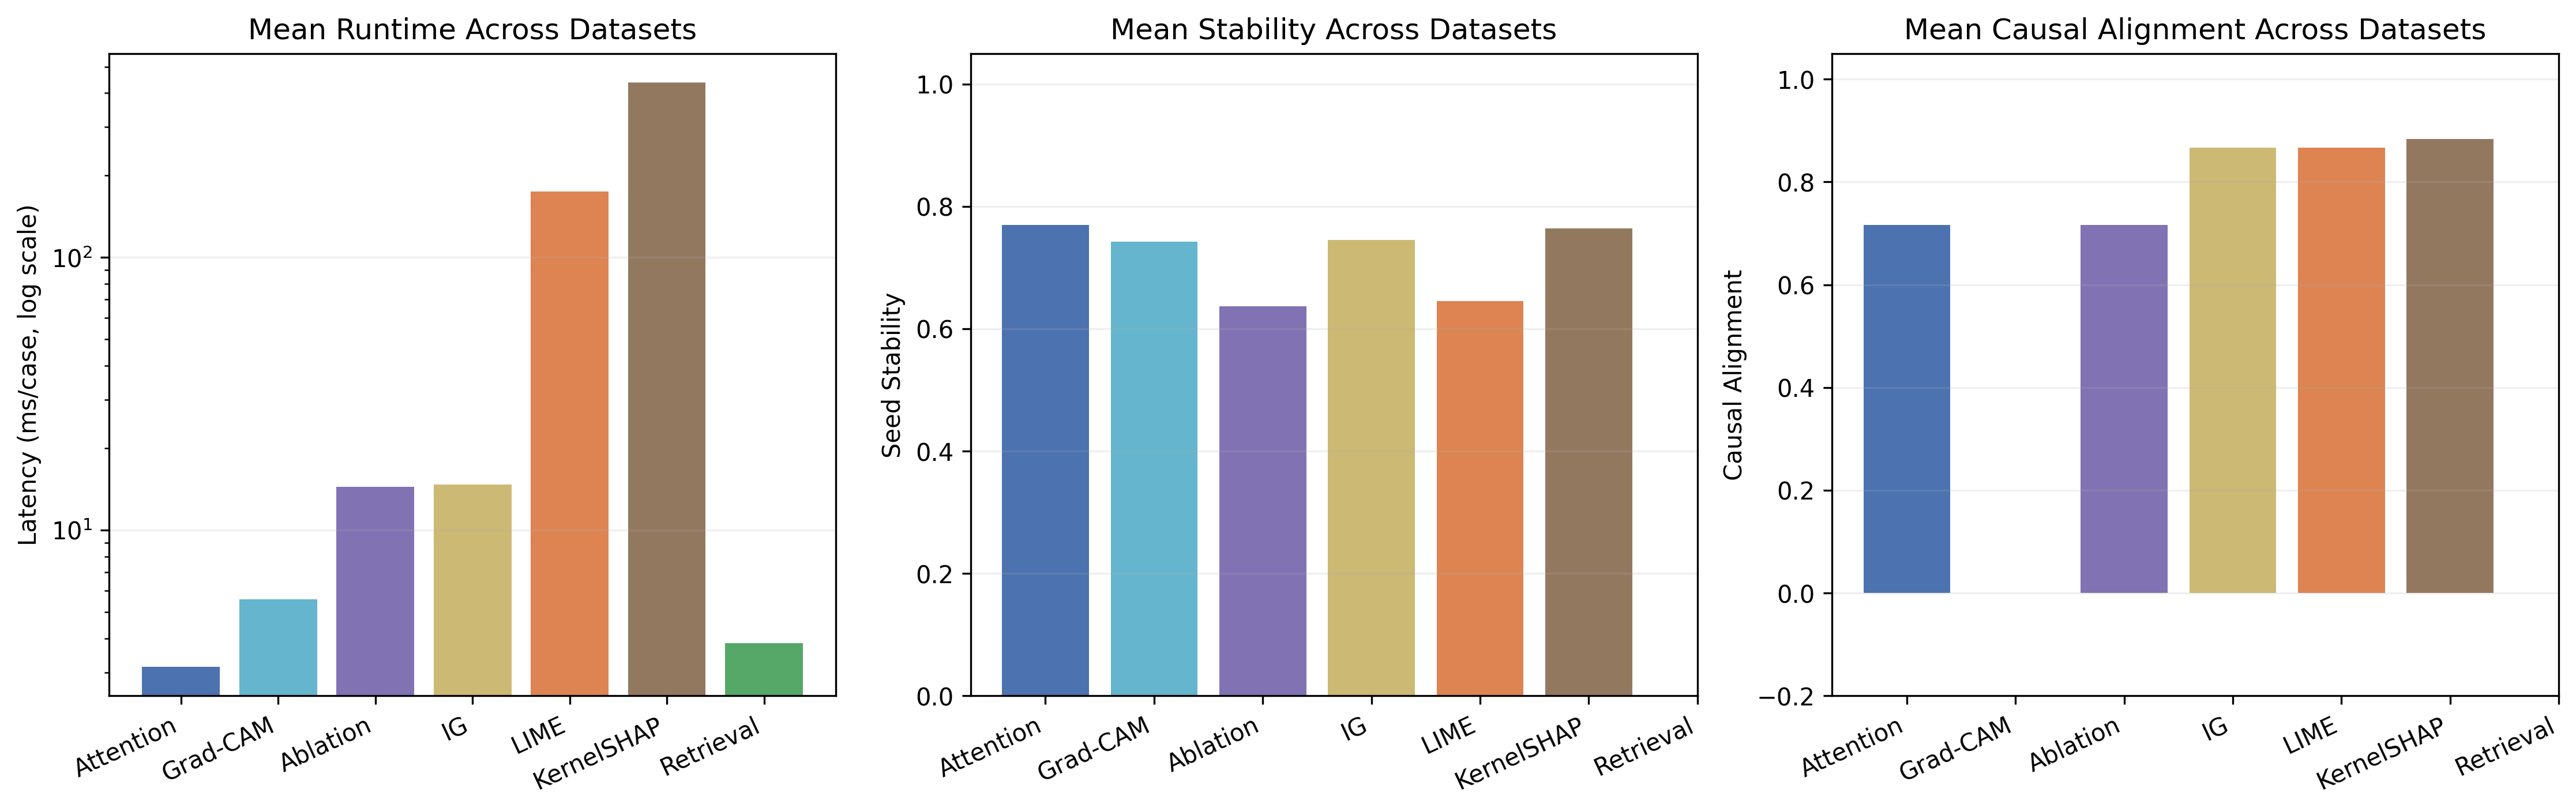
\includegraphics[width=\linewidth]{ace_suite_method_profile.png}
    \caption{Aggregate method profile across the six-domain ACE suite. Left: mean runtime. Middle: mean seed stability. Right: mean causal alignment.}
    \label{fig:ace_suite_method_profile}
\end{figure}

Figure \ref{fig:ace_suite_rank_consistency} makes the transportability claim explicit. The latency ranking was highly stable: attention was fastest on every dataset, followed by other intrinsic or lightweight methods. Causal-alignment leadership varied more by domain, alternating mainly between Integrated Gradients, KernelSHAP, and LIME, but the broad picture remained the same as in Table \ref{tab:method_suitability}: clinical usability depends on which action is being supported, not on a single global notion of ``best'' explanation.

\begin{figure}[h!]
    \centering
    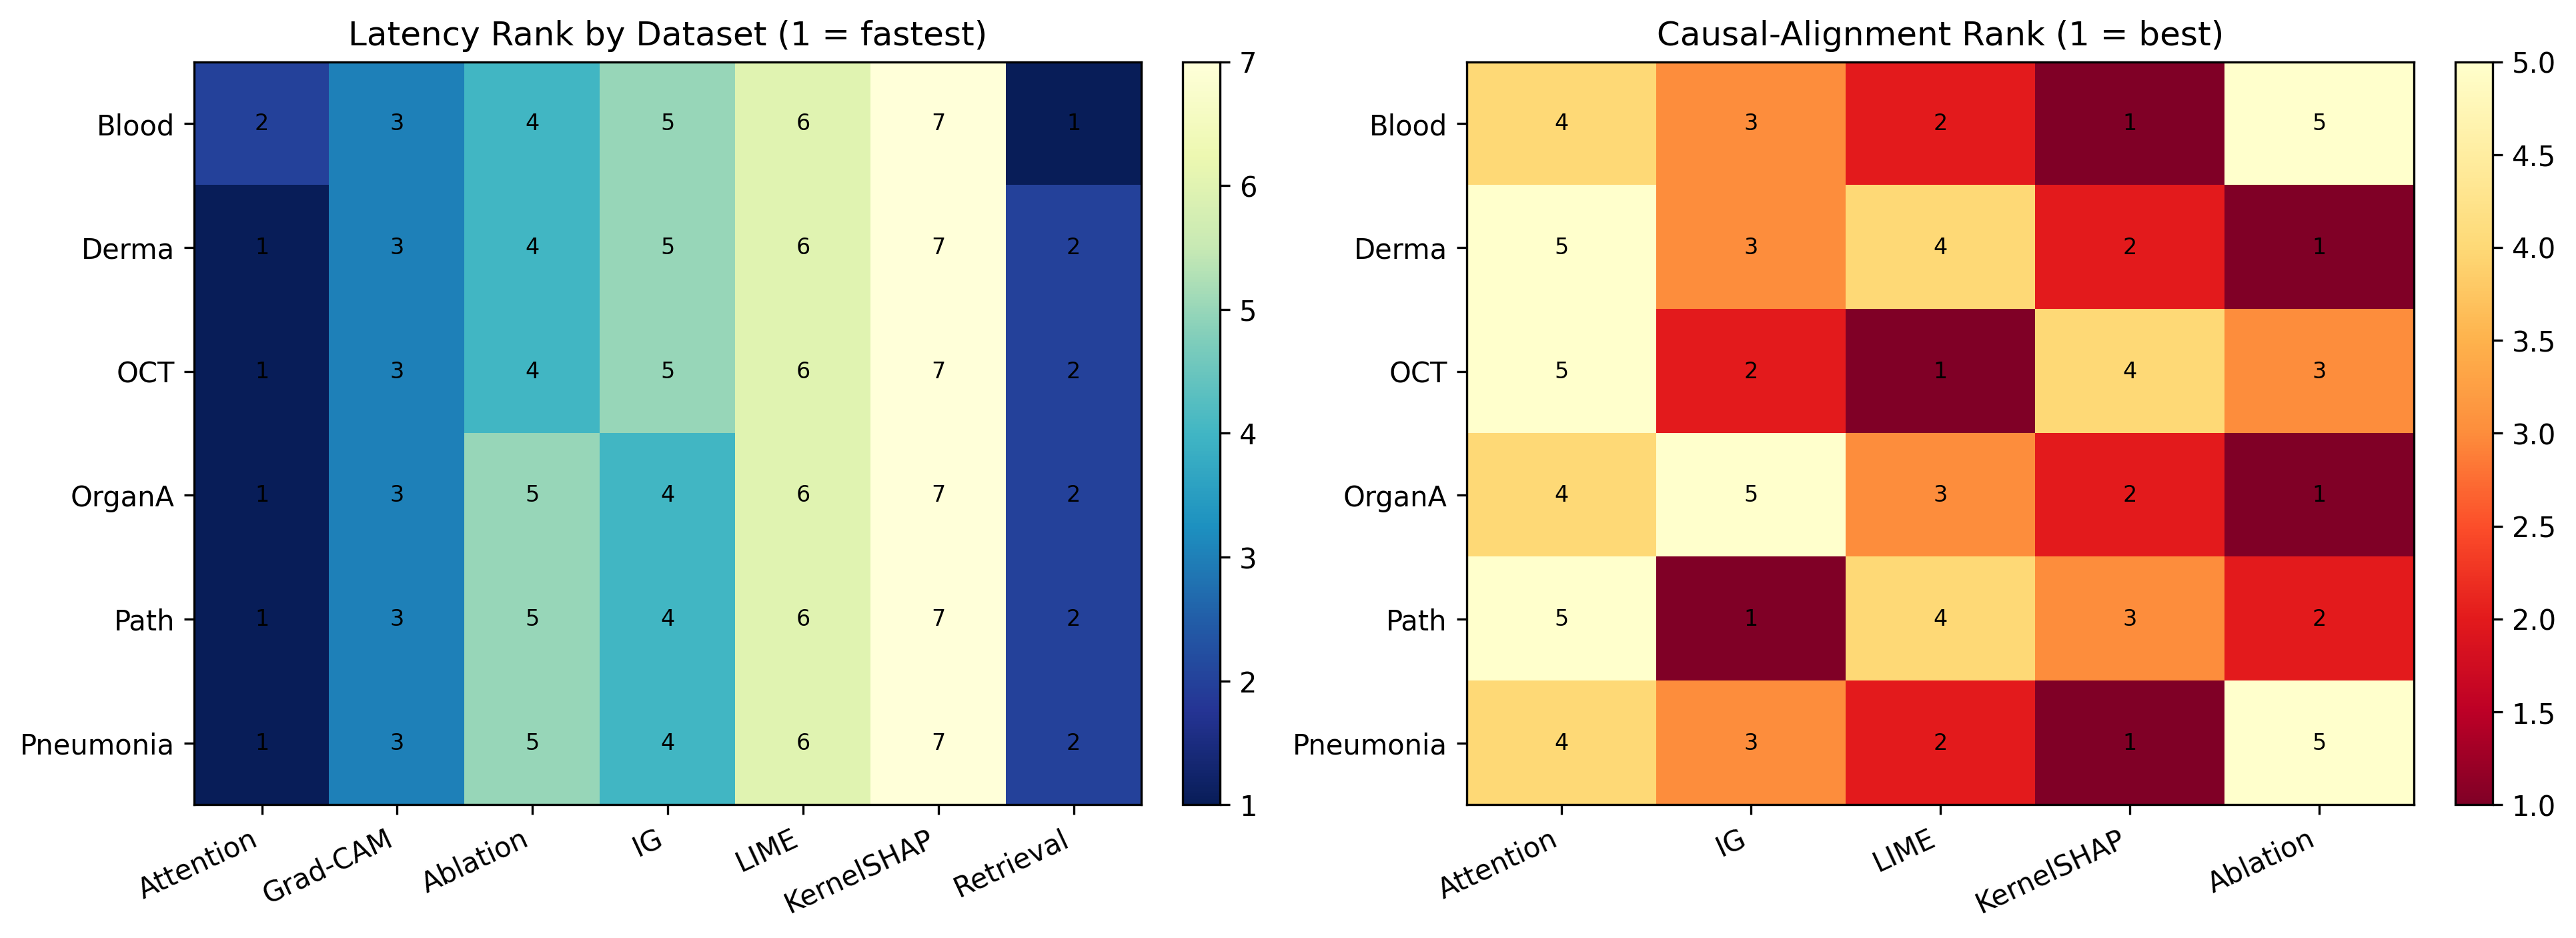
\includegraphics[width=\linewidth]{ace_suite_rank_consistency.png}
    \caption{Per-dataset rank consistency in the ACE suite. Left: latency rank (1 = fastest). Right: causal-alignment rank (1 = strongest alignment).}
    \label{fig:ace_suite_rank_consistency}
\end{figure}
Notably, causal-alignment leadership varies more across domains than latency ranking. In the cross-dataset suite, attention remains the fastest method on nearly all datasets, whereas the strongest causal-alignment scores alternate across methods: Integrated Gradients leads on OCTMNIST and PathMNIST, KernelSHAP leads on BloodMNIST and PneumoniaMNIST, and modality ablation leads on DermaMNIST and OrganAMNIST. This domain dependence reinforces the ACE argument that explanation suitability should be evaluated with respect to the target clinical action and data regime, rather than inferred from a single global ranking.

This larger public benchmark does not replace hospital-scale validation or reader studies, but it materially strengthens the survey's central operational claim: the trade-offs summarized in Table \ref{tab:method_suitability} are not artifacts of one dermatology benchmark. They recur across hematology, dermatology, retinal OCT, abdominal CT, histopathology, and chest X-ray tasks, making ACE a more transportable deployment rubric for multimodal medical XAI.

\section{Challenges and Future Directions}

This section highlights the open challenges in MXAI, including scalability, causality, fairness, the need for human-centric explanations, and the limitations of current methods. It also discusses promising future research directions, incorporating recent trends such as neuro-symbolic AI, federated learning, adversarial robustness, and the application of XAI to multimodal foundation models and time-series data.

\subsection{Limitations of the Present Work}
The ACE benchmark provides controlled, reproducible evidence but has four boundaries that must be stated explicitly.
Synthetic covariates and artificial shift. The spurious hospital feature was manually injected and randomized at test time. This controls the experimental conditions but does not reproduce the complexity of real clinical confounders, which are rarely this clean or well-defined.
Low-resolution architecture. All latency figures were measured on 28×28 images with a lightweight backbone. These are lower bounds. Full-resolution clinical pipelines (CT slices, whole-slide histopathology) will scale runtimes substantially, and the latency ranking across methods may not be fully preserved.
No clinician validation. No reader study was conducted. The benchmark measures technical properties — latency, causal alignment, seed stability — not whether clinicians find the explanations interpretable, actionable, or trustworthy in practice.
Single-institution, single-domain origin. Despite the six-domain cross-dataset extension, all experiments used synthetic multimodal augmentation of public datasets. Real multi-site variability, EHR integration, and federated deployment constraints are not captured. These boundaries define a clear validation roadmap. The next necessary steps are: (1) scaling the causal-invariance objective to full-resolution clinical pipelines to test whether the latency ranking holds at CT or whole-slide resolution; (2) conducting clinician reader studies to connect the technical ACE metrics to explanation usefulness in practice; and (3) extending the benchmark to real multi-site EHR data with naturalistic confounders. The controlled benchmark is offered not as a substitute for these steps, but as a reproducible foundation on which they can build.

\subsection{Open Challenges for the Field}

%\subsection{Systemic Failures of Model-Centric MXAI}

The ACE framework highlights three recurring deployment gaps:

\textbf{Failure 1: Regulatory Misalignment.} FDA lifecycle guidance emphasizes change management and validation for AI-enabled device software, while the EU AI Act foregrounds human oversight and accessible information \cite{fda2025draft,VANKOLFSCHOOTEN2024105152}. In practice, many MXAI papers still report static explanation snapshots without a protocol for revalidation after model updates or distribution shift.\newline 
%Figure \ref{fig:lifecycle_framework} discribes a typical workflow where this could fail.
Figure \ref{fig:lifecycle_framework} illustrates a typical healthcare AI lifecycle and highlights three points where current MXAI practice fails regulatory requirements: at training time, where causal validation is absent (Failure 1); at deployment, where explanation latency is unconstrained (Failure 2); and at monitoring, where no revalidation protocol exists after model updates (Failure 3). These three gaps motivate the research priorities detailed in Section 8.2
\textbf{Failure 2: Computational-Clinical Mismatch.} In teleoperation and remote surgery, end-to-end latency is itself a safety consideration \cite{anvari2005latency,moustris2023telesurgery5g}. Our controlled benchmark reinforces this point: perturbational explainers were 42--124$\times$ slower than intrinsic attention on the same lightweight multimodal model, even before scaling to larger clinical backbones.

\textbf{Failure 3: Clinical Validity Remains Weakly Tested.} Jin et al.\ showed that many explanation methods on a multimodal medical imaging task failed clinician-oriented requirements \cite{Jin_2022}, and recent human-centered evaluation surveys continue to report a gap between technical metrics and clinical usefulness \cite{gambetti2025surveyhumancenteredevaluationexplainable}. Our benchmark adds a complementary finding: cross-modal leakage and spurious feature reliance can persist even when several explanation methods look stable under simple seed-to-seed comparisons.
\begin{figure}[h!]
    \centering
    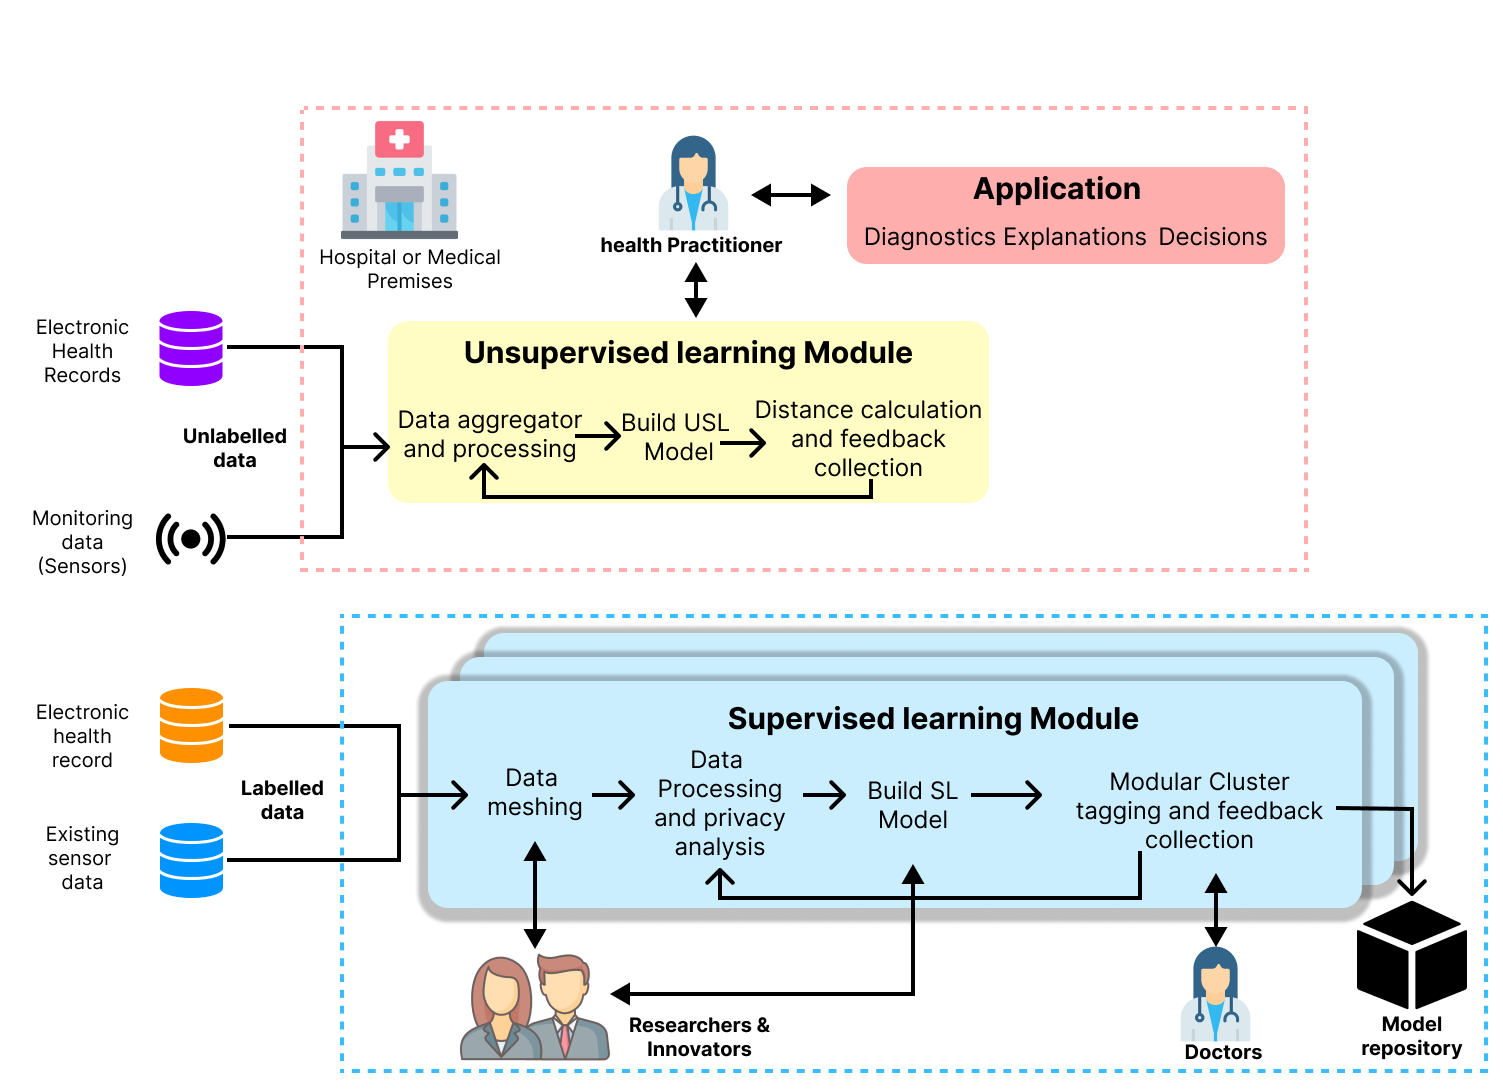
\includegraphics[width=0.97\linewidth]{Untitled.png}
    \caption{Lifecycle framework for healthcare Multimodal AI, illustrating the workflow from supervised training to clinical deployment and monitoring to ensure regulatory compliance}
    \label{fig:lifecycle_framework}
\end{figure}


\subsection{Research Priorities}
%{Future Directions (2025-2027)}
The three systemic failures identified in Section 8.1 directly motivate the following research priorities. Regulatory misalignment calls for regulatory-grade validation frameworks, primarily affecting the Audit and Monitoring actions under ACE. The computational-clinical mismatch calls for efficient explanation pipelines, most critical for Triage and Intraoperative Assistance. Finally, the weak clinical validity testing calls for causal attribution protocols, directly impacting Diagnosis and Treatment selection. Rather than listing generic directions, we detail each priority below in terms of its concrete research components.

\textbf{Regulatory-Grade XAI:} Develop explanation methods that satisfy both FDA transparency requirements and clinician usability. Priority: uncertainty-aware explanations with calibrated confidence intervals.
    
\textbf{Hallucination-Aware Deployment:} Integrate V-RAG with real-time validation against medical knowledge bases and clinician verification protocols. Research gap: balancing retrieval accuracy with latency in clinical settings.
    
\textbf{Standardized Clinical Benchmarks:} Expand benchmark coverage for rare disease categories, hard counterfactuals, and longitudinal drift, building on expert-driven resources such as SMMILE \cite{rieff2025smmileexpertdrivenbenchmarkmultimodal}.
    
\textbf{Structured Knowledge Integration:} Combine multimodal encoders with explicit retrieval, ontologies, or semantic layers to improve traceability and federated auditability \cite{info16060435}.
    
\textbf{Human-AI Teaming Protocols:} Shift from "AI as tool" to "AI as teammate" with dynamic explanation adjustment based on clinician expertise level and task complexity.

%\subsection{Priorities for Clinically Viable MXAI (2026--2027)}
%The evidence surveyed here suggests three immediate priorities:
%\textbf{1. Regulatory-Grade Validation Frameworks.}Develop \textit{explanation stress tests} that measure latency, clinician comprehension, calibration, and update-to-update stability under a unified protocol. Benchmarks such as SMMILE and human-centered evaluation frameworks provide important starting points, but not yet a complete lifecycle evaluation stack \cite{rieff2025smmileexpertdrivenbenchmarkmultimodal,gambetti2025surveyhumancenteredevaluationexplainable}.
%\textbf{2. Causal Attribution for Multimodal Models.} Move from correlational saliency toward intervention-aware validation. Early causal-intervention methods and causal reasoning benchmarks point in this direction, but clinically grounded counterfactual protocols remain limited \cite{chen2025causalclipsegunlockingclipspotential,li2025multimodalcausalreasoningbenchmark}.
%\textbf{3. Efficient Explanation Pipelines.}Deployment in time-sensitive workflows will require lightweight or partially precomputed explanation pathways. 

Our controlled benchmark showed a 42--124$\times$ runtime gap between perturbational explainers and intrinsic attention, which argues for approximation, distillation, caching, or retrieval-based evidence support rather than unconstrained online perturbation.

A key limitation of current MXAI evaluation is that fairness is usually measured only at the prediction level. Under ACE, fairness must also be action-specific and explanation-specific. For triage, fairness concerns whether urgent cases are prioritized consistently across subgroups; for diagnosis, whether equivalent clinical evidence receives equivalent explanatory weight; for treatment selection, whether counterfactual recommendations remain reliable across patient groups; for audit, whether subgroup-specific failures are traceable; and for monitoring, whether explanation drift is detected across sites and populations. 

Addressing these challenges and pursuing the outlined research directions will be crucial for advancing the field of MXAI and realizing its full potential in healthcare. By developing more scalable, robust, explainable, and human-centric MXAI systems, we can enhance the transparency, trustworthiness, and effectiveness of AI in improving patient care and driving medical innovation.

\section{Discussion}

This section synthesizes the key findings of the survey, reflects on the current state of MXAI, including its limitations, and highlights the most important open questions and future research opportunities.

The field of Multimodal Explainable AI (MXAI) has made significant strides in recent years, driven by the increasing need for transparency and trust in AI systems that integrate diverse data types. This survey has provided a comprehensive overview of the current state of MXAI, covering foundational concepts, methods, architectures, applications, datasets, evaluation metrics, and challenges, with a particular focus on the healthcare domain.

\subsection{Key Findings}
\textcolor{color}{The ACE framework reveals a fundamental tension in current MXAI practice: methods optimized for explanation fidelity, the dominant evaluation criterion in the literature, systematically fail on the properties that matter most for clinical deployment. No single method simultaneously achieves the latency constraints of triage, the causal validity required for diagnosis, the counterfactual reasoning needed for treatment, and the stability demanded for audit. This finding, confirmed across six medical domains in our cross-dataset benchmark, suggests that the field needs not better explainers per se, but better criteria for selecting among existing ones according to the clinical action being supported.}
%\begin{itemize}   \item \textbf{Action-Centered Framework:} The ACE taxonomy reveals that method classification by generation mechanism (ante-hoc/post-hoc) is clinically insufficient. Instead, explanations must be evaluated by their ability to support specific clinical decisions (triage, diagnosis, treatment, audit, monitoring), each with distinct safety-critical properties.
    %\item \textbf{Multimodal Architectures:} Transformers and attention mechanisms have become central to multimodal learning, while fusion networks and hybrid models offer alternative trade-offs between performance and interpretability \cite{rodis2024multimodalexplainableartificialintelligence,wani2024deepxplainer,HOFMANN2022119504}.
    %\item \textbf{Healthcare Applications:} The literature reviewed here shows broad use of MXAI in disease diagnosis, treatment support, and medical imaging analysis, with explainability serving both validation and communication roles in clinical workflows \cite{SADEGHI2024109370,Mohan_2025}.
%    \item \textbf{Evaluation Challenges:} Evaluating the quality of explanations remains difficult because ground truth is limited, metrics are often subjective, and technical scores do not always align with clinician-oriented requirements \cite{Jin_2022,gambetti2025surveyhumancenteredevaluationexplainable}.
 %   \item \textbf{Open Challenges:} Scalability, causality, fairness, and the need for human-centric explanations are major open challenges in MXAI. These challenges must be addressed to realize the full potential of MXAI in real-world applications.
%\end{itemize}


\subsection{Reflections on the Current State of MXAI}

%MXAI is a rapidly evolving field with the potential to revolutionize various domains, particularly healthcare, by making complex AI systems more transparent and understandable. While significant progress has been made in developing methods, architectures, and applications, MXAI is still in its early stages. Many current methods are computationally expensive, may not fully capture causal relationships, often produce explanations that are difficult for non-experts to understand, and are limited by the limitations described above.
The controlled benchmark reveals a more nuanced picture than the generic claim that MXAI methods are simply immature or unstable. In our setting, seed-to-seed instability was not the dominant failure mode: KernelSHAP, LIME, and Integrated Gradients all achieved stability scores above 0.82. Instead, the main empirical weakness was spurious multimodal reliance. \textcolor{red}{The baseline model showed a 0.252 mean generalization gap under the OOD hospital-shift setting}, and several explanation methods reflected this shortcut rather than clearly exposing it as non-causal. This suggests that stability alone is insufficient as a criterion for clinical explainability. Under ACE, intervention robustness and sensitivity to spurious cross-modal shortcuts should be evaluated alongside conventional explanation stability.

\subsection{\textcolor{red}{Clinical Expert review as Future Validation}}

 The present benchmark does not include clinician reader studies or prospective workflow evaluation. Therefore, the results should be interpreted as technical stress tests of ACE-relevant properties rather than evidence of clinical utility. A natural next step is an expert-review protocol in which clinicians assess randomized model explanations for representative ACE actions, rating interpretability, actionability, trust calibration, time-to-interpretation, and ability to detect spurious cues. Such a protocol would connect the technical metrics reported here to clinical usefulness and would help define action-specific acceptance thresholds. 


\subsection{Important Open Questions}

\begin{itemize}
    \item Our benchmark evaluated latency, stability, and causal alignment in isolation. No existing protocol combines these dimensions simultaneously under a unified regulatory framework
    \textbf{Regulatory-Grade Stress Testing:} How to develop unified protocols that measure latency, clinician comprehension, and stability simultaneously? Current benchmarks evaluate these in isolation, missing interaction effects.
    \item \textcolor{red}{Causal training reduced the mean generalization gap from 0.252 to 0.091 in the 500-case, 20-seed benchmark, but no ground-truth causal labels exist to formally validate whether the resulting explanations are causally correct.}
    \textbf{Causal Explanation Validation:} How to validate causal explanations against clinical ground truth? Existing evaluation practice still leaves a gap between technical metrics and clinician trust \cite{gambetti2025surveyhumancenteredevaluationexplainable}.
    \item No method evaluated in our benchmark produced confidence intervals on its own explanations, clinicians currently have no way to know when an explanation is unreliable.
    \textbf{Explanation Uncertainty Quantification:} How to provide confidence intervals for explanations themselves? Clinicians need to know \textit{when} an explanation is unreliable.
    
    \item  \textbf{Federated Explanation Consistency:} 
    How to maintain stable explanations across non-i.i.d. hospital data? Our benchmark operated on a single-institution setting, leaving open the question of whether ACE properties measured locally transfer across hospital sites. In one preliminary report on federated lung disease, explanation consistency degraded by 30–45\% \cite{Durga2025flem}, this single-study finding requires replication before drawing general conclusions.
        %How to maintain stable explanations across non-i.i.d. hospital data? In one federated lung disease setting, explanation consistency degraded by 30–45\% across non-i.i.d. hospital data [50] — a finding that warrants replication across broader MXAI contexts before drawing general conclusions \cite{Durga2025flem}.
\end{itemize}
Interdisciplinary collaboration is essential, but ACE provides a concrete basis for structuring it: AI researchers can optimize for the measurable properties (latency, causal alignment, stability) that clinicians and regulators need, rather than for abstract fidelity metrics that do not map to clinical actions.

%\textbf{Interdisciplinary collaboration} among AI researchers, clinicians, ethicists, and regulators is essential to develop MXAI systems that are powerful, transparent, and trustworthy.

\section{Conclusion}
%This survey introduced the Action-Centered Explainability (ACE) framework, which reframes MXAI evaluation around five clinical actions, triage, diagnosis, treatment selection, audit, and monitoring, each associated with distinct and measurable explanation requirements. By shifting from algorithmic classification to decision-oriented evaluation, ACE exposes a fundamental limitation of current practice: no single explanation method simultaneously satisfies the latency, causal validity, stability, and traceability requirements across all clinical actions.


%This survey argues that the central limitation of current MXAI practice is a \textit{taxonomic misalignment}---organizing explanation methods by algorithmic family rather than by the clinical actions they must support. By introducing the Action-Centered Explainability (ACE) framework and grounding it in a controlled multimodal benchmark, we show that different actions require different explanation properties: attention and Grad-CAM are attractive for low-latency workflows, modality ablation is stronger for intervention-style reasoning and drift exposure, and perturbational methods such as LIME and KernelSHAP remain substantially slower even on a lightweight benchmark. 

%\textcolor{red}{The strongest empirical signal in our experiments was not random explanation drift, but spurious multimodal reliance: in the 500-case, 20-seed benchmark, a causal-invariance objective improved mean OOD accuracy from 0.604 to 0.753 and reduced the mean generalization gap from 0.252 to 0.091.}

%The resulting message is practical: MXAI should be judged less by whether an explainer is ante-hoc or post-hoc, and more by whether it is fast enough, stable enough, intervention-aware enough, and traceable enough for the clinical action at hand. 

%Emerging directions---including neuro-symbolic AI, causal training, retrieval-grounded evidence, federated validation, and foundation-model explainability---offer plausible next steps, but their value will depend on whether they are evaluated under the same action-centered stress tests. Realizing MXAI's potential therefore requires not only better explanations, but better experimental protocols for proving when those explanations are clinically actionable, legally defensible, and safe.
%Among the emerging directions surveyed, three are most urgently motivated by the ACE findings: efficient explanation pipelines to close the 42--124$\times$ latency gap between perturbational and intrinsic methods, causal attribution protocols to move beyond correlational saliency, and regulatory-grade validation frameworks to align MXAI evaluation with FDA lifecycle requirements.
%The ACE framework provides a structured basis for this effort: by making the requirements of each clinical action explicit and measurable, it offers AI researchers, clinicians, and regulators a common language for deciding not just which explanation method to use, but whether any current method is ready for deployment in a given clinical context.

This survey introduced the Action-Centered Explainability (ACE) framework, which reframes MXAI evaluation around five clinical actions-triage, diagnosis, treatment selection, audit, and monitoring each associated with distinct and measurable explanation requirements. By shifting from algorithmic classification to decision-oriented evaluation, ACE exposes a structural limitation of current practice: no single explanation method simultaneously satisfies the latency, causal validity, stability, and traceability requirements that span all clinical actions.
The dominant empirical signal was not abstract explanation instability, but spurious multimodal reliance: in a 500-case, 20-seed benchmark, a causal-invariance objective improved mean OOD accuracy from 0.604 to 0.753 and reduced the mean generalization gap from 0.252 to 0.091, not by improving the explainer, but by improving what the model had learned to rely on. This finding argues that explanation quality cannot be decoupled from training-time causal discipline.
Three research priorities are most urgently motivated by these findings: Efficient explanation pipelines to close the 42–124× latency gap between perturbational and intrinsic methods, without sacrificing causal alignment; Causal attribution protocols to move beyond correlational saliency and toward interventionally valid explanations suitable for diagnosis and treatment selection; and regulatory-grade validation frameworks to align MXAI evaluation with FDA lifecycle requirements and EU AI Act transparency obligations.
ACE does not resolve these challenges, it structures them. By making the requirements of each clinical action explicit and measurable, the framework provides AI researchers, clinicians, and regulators with a common language for deciding not just which explanation method to use, but whether any current method is genuinely ready for deployment in a given clinical context.







%%===========================================================================================%%
%% If you are submitting to one of the Nature Portfolio journals, using the eJP submission   %%
%% system, please include the references within the manuscript file itself. You may do this  %%
%% by copying the reference list from your .bbl file, paste it into the main manuscript .tex %%
%% file, and delete the associated \verb+\bibliography+ commands.                            %%
%%===========================================================================================%%

\bibliography{sn-bibliography}% common bib file
%% if required, the content of .bbl file can be included here once bbl is generated
%%\input sn-article.bbl

\end{document}

